\documentclass[11pt,a4paper]{article}
\usepackage[utf8]{inputenc}
\usepackage[T1]{fontenc}
\usepackage[spanish,es-noshorthands,es-tabla]{babel}
\usepackage{lmodern}
\usepackage[margin=2.3cm]{geometry}
\usepackage{graphicx}
\usepackage{booktabs,longtable,tabularx,array,multirow}
\usepackage{enumitem}
\usepackage[table]{xcolor}
\usepackage{pdflscape}
\usepackage{afterpage}
\usepackage{tikz}
\usetikzlibrary{shapes.geometric,positioning}
\usepackage{amssymb}
\usepackage{float}
\usepackage{caption}
\usepackage[hidelinks]{hyperref}
\usepackage{fancyhdr}
\usepackage{listings}
% =====================================================================
% Estilo y comandos del Hito 2 (se carga desde informe_hito2.tex)
% =====================================================================

% Código SQL y salidas de PostgreSQL
\definecolor{codigofondo}{HTML}{F6F6F4}
\definecolor{codigocoment}{HTML}{6B6A66}
\definecolor{codigoclave}{HTML}{1C5CAB}
\lstdefinestyle{sql}{
  language=SQL, basicstyle=\ttfamily\footnotesize, keywordstyle=\color{codigoclave}\bfseries,
  commentstyle=\color{codigocoment}\itshape, backgroundcolor=\color{codigofondo},
  frame=single, rulecolor=\color{codigofondo}, breaklines=true, columns=fullflexible,
  showstringspaces=false, upquote=true, tabsize=2,
  morekeywords={RETURNING,LATERAL,FILTER,OVER,PARTITION,EXCLUDE,USING,INCLUDE,BRIN,GIST,
                REPLACE,PROCEDURE,TRIGGER,FUNCTION,RETURNS,LANGUAGE,DECLARE,BEGIN,RAISE,EXCEPTION,
                IF,THEN,ELSIF,END,CALL,INOUT,DEFERRABLE,INITIALLY,DEFERRED,EXECUTE,ROLE,GRANT,REVOKE,
                EXPLAIN,ANALYZE,VACUUM,WITH,RECURSIVE,COALESCE,EXTRACT,EPOCH,SERIAL,TIMESTAMP,BOOLEAN},
  literate={á}{{\'a}}1 {é}{{\'e}}1 {í}{{\'i}}1 {ó}{{\'o}}1 {ú}{{\'u}}1 {ñ}{{\~n}}1
           {Á}{{\'A}}1 {É}{{\'E}}1 {Í}{{\'I}}1 {Ó}{{\'O}}1 {Ú}{{\'U}}1 {Ñ}{{\~N}}1
           {°}{{\textdegree}}1 {×}{{$\times$}}1 {≥}{{$\geq$}}1 {≤}{{$\leq$}}1 {→}{{$\rightarrow$}}1
}
\lstdefinestyle{salida}{
  basicstyle=\ttfamily\scriptsize, backgroundcolor=\color{codigofondo}, frame=single,
  rulecolor=\color{codigofondo}, breaklines=true, columns=fullflexible, showstringspaces=false,
  literate={á}{{\'a}}1 {é}{{\'e}}1 {í}{{\'i}}1 {ó}{{\'o}}1 {ú}{{\'u}}1 {ñ}{{\~n}}1
           {Ú}{{\'U}}1 {°}{{\textdegree}}1 {→}{{$\rightarrow$}}1 {×}{{$\times$}}1
}

% Resultados del experimento (los genera bench/experimento.py en informe/resultados/)
\newcommand{\resdir}{resultados}
\newcommand{\pendiente}[1]{\fbox{\parbox{0.9\linewidth}{\centering\small Pendiente: ejecutar
  \texttt{bench/experimento.py} para generar \texttt{\detokenize{#1}}.}}}
\newcommand{\entrada}[1]{\IfFileExists{\resdir/#1}{\input{\resdir/#1}}{\pendiente{#1}}}
\newcommand{\grafico}[2]{\IfFileExists{\resdir/graficos/#1}%
  {\includegraphics[width=#2\linewidth]{\resdir/graficos/#1}}{\pendiente{graficos/#1}}}
\newcommand{\plan}[1]{\IfFileExists{\resdir/planes/#1}%
  {\lstinputlisting[style=salida]{\resdir/planes/#1}}{\pendiente{planes/#1}}}
% Versión corta del plan (bench/resumir_planes.py): solo nodos, filas y tiempo
\newcommand{\planresumen}[1]{\IfFileExists{\resdir/planes_resumen/#1}%
  {\lstinputlisting[style=salida]{\resdir/planes_resumen/#1}}{\pendiente{planes_resumen/#1}}}
\newcommand{\archivo}[1]{\texttt{\detokenize{#1}}}

\pagestyle{fancy}
\fancyhf{}
\fancyhead[L]{\small CS2041 -- UTEC\\ \small Base de Datos I}
\fancyhead[C]{\small 2026-2}
\fancyhead[R]{\small Proyecto Final -- Hito 2\\ \small Grupo 3 -- Tópico 4}
\fancyfoot[C]{\thepage}
\renewcommand{\headrulewidth}{0.4pt}
\setlength{\headheight}{26pt}

\setlist{itemsep=2pt,topsep=4pt}
\setlength{\parskip}{4pt}
\renewcommand{\arraystretch}{1.15}

% Notación del modelo relacional
\newcommand{\pk}[1]{\underline{#1}}
\newcommand{\fk}[1]{\textit{#1}\textsuperscript{\tiny FK}}
\newcommand{\pkfk}[1]{\underline{\textit{#1}}\textsuperscript{\tiny FK}}
\newcommand{\tb}[1]{\textbf{\texttt{#1}}}
\newcommand{\at}[1]{\texttt{#1}}

\begin{document}
\sloppy

% ---------------------------------------------------------------- Portada
\begin{titlepage}
\centering
{\large Universidad de Ingeniería y Tecnología -- UTEC\par}
\vspace{0.4cm}
{\large CS2041 Base de Datos I -- Ciclo 2026-2\par}
\vspace{2.5cm}
{\LARGE\bfseries Proyecto Final -- Hito 2\par}
\vspace{0.6cm}
{\Huge\bfseries SkyNest\par}
\vspace{0.3cm}
{\Large Sistema de base de datos para la gestión de drones\\ de envíos urbanos en Lima Metropolitana\par}
\vspace{0.6cm}
{\large Tópico 4: Gestión de Drones para Envíos Urbanos\par}
\vspace{2.5cm}
{\large\bfseries Grupo 3\par}
\vspace{0.3cm}
\begin{tabular}{l}
Saquiray Delgado, Samuel Aaron -- 202310697 \\
Caceres Sanchez, Matias Andres -- 202510370 \\
Del Negro Yabar, Giuseppe Antonio -- 202110545 \\
\end{tabular}
\vfill
{\large Profesor: Wilder Nina\par}
\vspace{0.3cm}
{\large Lima, \today\par}
\end{titlepage}

\tableofcontents
\newpage

% ================================================================ 1
\section{Requisitos}

\subsection{Introducción}
El reparto de última milla es el tramo más caro y lento de la cadena logística urbana. En Lima Metropolitana, la congestión vehicular hace que un envío de pocos kilómetros pueda tardar más de una hora por tierra. Los drones de reparto, que vuelan en línea recta sobre el tráfico, permiten entregar paquetes livianos (medicamentos, repuestos, documentos, muestras de laboratorio o compras de comercio electrónico) en minutos.

Operar una flota de drones exige, sin embargo, un control de información mucho más estricto que el de una flota de motos: cada vuelo debe estar asociado a un drone registrado, a una ruta aprobada, a un operador con licencia vigente y a una batería en buen estado, y cada batería emite telemetría continua que determina si el vuelo puede continuar con seguridad. Este documento especifica los requisitos de la base de datos que soportará dicha operación.

\subsection{Descripción general del problema/organización/empresa}
\textbf{SkyNest} es una empresa (ficticia, planteada para este proyecto) de reparto urbano con drones que opera en Lima Metropolitana y el Callao. Su infraestructura se organiza en:

\begin{itemize}
\item \textbf{Estaciones nest}: bases físicas ubicadas en azoteas o terrenos de distintos distritos, donde los drones despegan, aterrizan, se estacionan y recargan o intercambian baterías. Cada nest tiene una capacidad máxima de drones y un número de puertos de carga.
\item \textbf{Flota de drones}: aeronaves pilotadas a distancia (RPAS) de distintos modelos y fabricantes, cada una registrada ante la autoridad aeronáutica y asignada a un nest base.
\item \textbf{Baterías}: unidades intercambiables que se instalan y retiran de los drones; su estado de salud se degrada con los ciclos de carga.
\item \textbf{Operadores}: pilotos certificados que supervisan los vuelos desde un nest (un operador puede supervisar varios vuelos autónomos en paralelo).
\item \textbf{Clientes}: personas naturales y empresas (farmacias, laboratorios, tiendas) que registran paquetes para envío.
\item \textbf{Rutas de vuelo}: corredores aéreos aprobados que salen de un nest hacia un distrito de destino, definidos por una secuencia ordenada de puntos de paso (waypoints).
\end{itemize}

El problema a resolver es que hoy la información de estas piezas está dispersa y no existe un registro único y consistente que permita saber, para cada entrega, qué drone la hizo, con qué batería, por qué ruta, bajo la supervisión de quién y cómo se comportó la batería durante el vuelo.

\subsection{Necesidad/usos de la base de datos}
La base de datos debe servir como fuente única de verdad para la operación. Sus usos principales son:

\begin{enumerate}
\item \textbf{Despacho}: asignar paquetes pendientes a vuelos, verificando que el peso total no supere la carga útil del modelo de drone y que el drone, la batería y el operador estén disponibles y habilitados.
\item \textbf{Seguimiento}: consultar el estado de un paquete a partir de su código de tracking y conocer el vuelo que lo transporta.
\item \textbf{Seguridad operacional}: almacenar la telemetría de baterías (voltaje, corriente, temperatura y porcentaje de carga) para detectar sobrecalentamientos, descargas anómalas o baterías degradadas antes de que causen un incidente.
\item \textbf{Mantenimiento}: llevar el historial de uso de cada batería (en qué vuelos y drones se usó), los ciclos de carga y el estado de salud de cada batería, así como las horas de vuelo acumuladas de cada drone.
\item \textbf{Cumplimiento normativo}: conservar la trazabilidad de cada vuelo (drone registrado, operador con licencia vigente y autorizado para el modelo de drone y el distrito, ruta aprobada) exigida por la regulación peruana de RPAS (Ley N.° 30740 y la NTC 001-2015 de la DGAC).
\item \textbf{Análisis del negocio}: medir la tasa de entregas exitosas por nest y por distrito, los tiempos de entrega, la utilización de la flota y el consumo energético por modelo y ruta.
\end{enumerate}

\subsection{¿Cómo resuelve el problema hoy?}

\subsubsection{¿Cómo se almacenan/procesan los datos hoy?}
En la situación actual (fase piloto), la información se maneja de forma fragmentada:

\begin{itemize}
\item Los paquetes se registran en un formulario web cuyas respuestas llegan a una hoja de cálculo compartida.
\item La asignación de paquetes a drones la decide manualmente el operador de turno y se anota en otra hoja por nest.
\item La telemetría de cada vuelo queda en los archivos de log que genera la estación de control de cada drone (archivos CSV o binarios del fabricante), guardados en carpetas por fecha, sin vínculo con el paquete ni con el operador.
\item El inventario de drones y baterías, junto con los registros ante la DGAC y las licencias de los operadores, se lleva en documentos separados.
\end{itemize}

Esto provoca duplicidad de datos, errores de digitación (códigos de tracking repetidos, pesos mal registrados), imposibilidad de responder preguntas que cruzan fuentes (por ejemplo, ``¿qué baterías se sobrecalentaron en vuelos hacia San Isidro el último mes?'') y riesgo de volar con una batería degradada o con un operador cuya licencia ya venció.

\subsubsection{Flujo de datos}
El flujo de información de un envío, que el sistema debe soportar de extremo a extremo, es el siguiente:

\begin{enumerate}
\item El cliente (persona o empresa) registra un paquete indicando peso, dimensiones, destinatario y dirección de destino. Se genera un código de tracking y el paquete queda en estado \at{registrado}.
\item El sistema determina el distrito de destino y el nest de origen más conveniente; el despachador programa un \emph{vuelo} que usa una ruta aprobada desde ese nest hacia ese distrito, con un drone disponible del nest y un operador asignado.
\item Al programar el vuelo se le asigna la batería cargada que usará el drone; el sistema verifica que la batería esté operativa y que el operador esté autorizado para ese modelo de drone en el distrito de destino.
\item Los paquetes se asignan al vuelo (estado \at{asignado}) y, al despegar, pasan a \at{en\_ruta}.
\item Durante el vuelo, cada batería envía lecturas de telemetría periódicas (por ejemplo, cada 5 segundos), que se insertan en la base de datos.
\item Al completar la entrega, el paquete pasa a \at{entregado} con su fecha y hora de entrega (o a \at{fallido}/\at{devuelto} si no se pudo entregar). El vuelo se cierra con su hora de aterrizaje y distancia real, y se actualizan las horas de vuelo del drone.
\item Al retirar la batería se registra la fecha de retiro, y se actualizan sus ciclos de carga y su estado de salud.
\item Periódicamente, los analistas consultan indicadores agregados (entregas por distrito, tiempos, consumo de batería, utilización de la flota).
\end{enumerate}

\subsection{Descripción detallada del sistema}

\subsubsection{Objetos de información actuales}
\begin{itemize}
\item \textbf{Distrito}: distritos de Lima Metropolitana y el Callao identificados por su código UBIGEO del INEI; indica si el espacio aéreo está restringido (por ejemplo, cerca del aeropuerto) y la altitud máxima permitida.
\item \textbf{Estación nest}: código, nombre, dirección, coordenadas, capacidad de drones, puertos de carga y estado operativo.
\item \textbf{Modelo de drone}: fabricante, nombre comercial, carga útil máxima, autonomía, velocidad de crucero, alcance y número de baterías que usa simultáneamente.
\item \textbf{Drone}: número de serie, código de registro ante la DGAC, fecha de adquisición, estado y horas de vuelo acumuladas.
\item \textbf{Batería}: número de serie, química, capacidad, voltaje nominal, ciclos de carga, estado de salud (SoH) y estado.
\item \textbf{Autorización de operación}: permiso que habilita a un operador a volar un modelo de drone determinado sobre un distrito determinado, con fechas de emisión y vencimiento.
\item \textbf{Operador}: DNI, nombres, contacto, número de licencia de piloto RPAS y su fecha de vencimiento.
\item \textbf{Cliente}: datos de contacto; si es persona natural, DNI y nombres; si es empresa, RUC y razón social.
\item \textbf{Paquete}: código de tracking, peso, dimensiones, prioridad, fragilidad, destinatario, dirección y coordenadas de destino, estado, fechas y costo del envío.
\item \textbf{Ruta de vuelo}: código, nest de origen, distrito de destino, distancia, altitud de crucero, duración estimada y si está activa.
\item \textbf{Punto de ruta}: waypoints ordenados de la ruta (latitud, longitud, altitud y tipo).
\item \textbf{Vuelo}: ejecución concreta de una ruta por un drone bajo la supervisión de un operador, con horarios programado y reales, estado y distancia recorrida.
\item \textbf{Telemetría de batería}: lecturas periódicas de voltaje, corriente, temperatura y porcentaje de carga de una batería durante un vuelo.
\end{itemize}

\subsubsection{Características y funcionalidades esperadas}
\begin{itemize}
\item Registro y actualización de clientes, paquetes, drones, baterías, nests, rutas y operadores.
\item Programación de vuelos con validaciones automáticas: drone disponible, operador con licencia vigente, ruta activa, peso total dentro de la carga útil y batería con salud suficiente.
\item Ingesta masiva y continua de telemetría con inserciones rápidas.
\item Seguimiento de paquetes por código de tracking en tiempo casi real.
\item Historial completo de uso de baterías por vuelo y por drone, y registro de autorizaciones de operadores por modelo y distrito.
\item Actualización automática (triggers, a implementar en el Hito 2) de estados: paquete al despegar y aterrizar el vuelo, horas de vuelo del drone, ciclos de la batería, y bloqueo de baterías degradadas.
\item Reportes y vistas de indicadores: entregas por distrito y nest, tiempos de entrega frente a lo estimado, consumo de batería por modelo y ruta, utilización de la flota y alertas de temperatura.
\end{itemize}

\subsubsection{Tipos de usuarios existentes/necesarios}
\begin{center}
\begin{tabularx}{\textwidth}{>{\bfseries}l X}
\toprule
Usuario & Permisos y uso principal \\
\midrule
Administrador & Control total: gestiona nests, modelos, drones, baterías, rutas, operadores y usuarios de la base de datos. \\
Despachador & Programa vuelos, asigna paquetes y baterías a vuelos. \\
Operador (piloto) & Consulta los vuelos que supervisa, actualiza su estado (despegue, aterrizaje, aborto) y ve la telemetría en vivo. \\
Cliente & Registra paquetes y consulta únicamente el estado de sus propios envíos. \\
Técnico de mantenimiento & Consulta la telemetría y el historial de baterías y drones, y actualiza su salud y estado. \\
Analista & Acceso de solo lectura a vistas agregadas para reportes de gestión. \\
Sistema de telemetría & Usuario técnico que solo puede insertar lecturas en la tabla de telemetría. \\
\bottomrule
\end{tabularx}
\end{center}

\subsubsection{Tipos de consulta, actualizaciones}
\paragraph{Actualizaciones y frecuencia.}
\begin{itemize}
\item \textbf{Carga estática (una vez, con cambios esporádicos)}: distritos (UBIGEO), modelos de drone, nests, rutas y sus puntos.
\item \textbf{Cambios ocasionales (semanales/mensuales)}: alta y baja de drones, baterías y operadores; renovación de licencias y autorizaciones; activación o desactivación de rutas.
\item \textbf{Cambios diarios (transaccionales)}: registro de clientes y paquetes, programación de vuelos, asignación de baterías, cambios de estado de paquetes y vuelos.
\item \textbf{Alta frecuencia (continua)}: inserción de lecturas de telemetría durante cada vuelo. Es la tabla de mayor crecimiento y es de solo inserción (no se modifica ni se borra).
\end{itemize}

\paragraph{Consultas esperadas.} Se prevén consultas como las siguientes; de ellas se seleccionarán las 5 consultas intermedias del Hito 2:
\begin{enumerate}
\item Estado y vuelo actual de un paquete a partir de su código de tracking (consulta puntual y muy frecuente).
\item Tasa de entregas exitosas y tiempo promedio de entrega por nest de origen y distrito de destino en un rango de fechas.
\item Consumo promedio de batería (puntos porcentuales de carga por kilómetro) por modelo de drone y ruta.
\item Baterías con lecturas de temperatura por encima de un umbral o caídas de voltaje anómalas en los últimos $N$ vuelos, junto con los drones que las usaron.
\item Utilización de la flota: horas voladas y número de vuelos por drone y por nest en el mes, comparadas con el promedio de su modelo.
\item Paquetes \emph{express} entregados con retraso respecto de la duración estimada de la ruta, agrupados por distrito.
\item Clientes con mayor volumen de envíos y facturación por mes.
\item Operadores con licencia por vencer en los próximos 30 días y los vuelos que tienen programados.
\end{enumerate}

\paragraph{Tiempos de respuesta esperados.}
\begin{center}
\begin{tabular}{lc}
\toprule
Operación & Tiempo objetivo \\
\midrule
Inserción de una lectura de telemetría & $< 10$ ms \\
Búsqueda de paquete por código de tracking & $< 50$ ms \\
Registro de paquete / programación de vuelo (con validaciones) & $< 200$ ms \\
Consultas analíticas intermedias sobre 1 millón de registros & $< 2$ s \\
Reportes mensuales agregados & $< 10$ s \\
\bottomrule
\end{tabular}
\end{center}

\subsubsection{Tamaño estimado de la base de datos}
La estimación considera un año de operación con 30 nests y unos 2\,500 envíos diarios. Una lectura de telemetría cada 5 segundos, en vuelos de unos 15 minutos, genera alrededor de 180 lecturas por vuelo.

Para estimar el espacio se sumó la longitud de los atributos de cada tabla, usando el tamaño de los tipos de PostgreSQL: 4 bytes para \texttt{INTEGER}/\texttt{SERIAL} y \texttt{DATE}, 8 para \texttt{TIMESTAMP} y \texttt{NUMERIC}, 2 para \texttt{SMALLINT}, 1 para \texttt{BOOLEAN}, $n$ para \texttt{CHAR($n$)} y $n+1$ para \texttt{VARCHAR($n$)} en el peor caso. La Tabla~\ref{tab:bytes1} muestra la longitud de un registro por tabla y la Tabla~\ref{tab:bytes2} el espacio total estimado.

\begin{table}[H]
\centering\small
\caption{Longitud estimada de un registro por tabla.}
\label{tab:bytes1}
\begin{tabular}{l l r}
\toprule
Tabla & Longitud de los atributos (bytes) & Registro (bytes) \\
\midrule
\tb{distrito} & 6+61+31+1+8 & 107 \\
\tb{estacion\_nest} & 4+13+81+151+8+8+2+2+16+6 & 291 \\
\tb{modelo\_drone} & 4+51+51+8+2+8+8 & 132 \\
\tb{drone} & 4+31+21+4+16+8+4+4 & 92 \\
\tb{bateria} & 4+31+11+4+8+4+8+13 & 83 \\
\tb{operador} & 4+8+61+61+101+16+21+4+4 & 280 \\
\tb{autorizacion} & 4+4+6+4+4 & 22 \\
\tb{cliente} & 4+101+16+8 & 129 \\
\tb{cliente\_persona} & 4+8+61+61 & 134 \\
\tb{cliente\_empresa} & 4+11+121+81 & 217 \\
\tb{ruta\_vuelo} & 4+16+4+6+8+8+2+1 & 49 \\
\tb{punto\_ruta} & 4+2+8+8+8+13 & 43 \\
\tb{permiso\_vuelo} & 4+21+6+4+4+13 & 52 \\
\tb{vuelo} & 4+4+4+4+4+4+8+8+8+13+11+8 & 80 \\
\tb{paquete} & 4+12+4+4+6+8+8+8+8+11+1+101+16+151+8+8+13+8+8+8 & 395 \\
\tb{telemetria\_bateria} & 4+8+8+8+8+8 & 44 \\
\bottomrule
\end{tabular}
\end{table}

\begin{table}[H]
\centering\small
\caption{Espacio estimado para un año de operación.}
\label{tab:bytes2}
\begin{tabular}{l r r r l}
\toprule
Tabla & Registro (B) & Registros & Total (bytes) & Crecimiento \\
\midrule
\tb{distrito} & 107 & 50 & 5\,350 & Estático \\
\tb{estacion\_nest} & 291 & 30 & 8\,730 & Casi estático \\
\tb{modelo\_drone} & 132 & 8 & 1\,056 & Casi estático \\
\tb{drone} & 92 & 300 & 27\,600 & Lento \\
\tb{bateria} & 83 & 900 & 74\,700 & Lento \\
\tb{operador} & 280 & 120 & 33\,600 & Lento \\
\tb{autorizacion} & 22 & 1\,500 & 33\,000 & Lento \\
\tb{cliente} & 129 & 60\,000 & 7\,740\,000 & Moderado \\
\tb{cliente\_persona} & 134 & 45\,000 & 6\,030\,000 & Moderado \\
\tb{cliente\_empresa} & 217 & 15\,000 & 3\,255\,000 & Moderado \\
\tb{ruta\_vuelo} & 49 & 600 & 29\,400 & Lento \\
\tb{punto\_ruta} & 43 & 6\,000 & 258\,000 & Lento \\
\tb{permiso\_vuelo} & 52 & 2\,000 & 104\,000 & Lento \\
\tb{vuelo} & 80 & 600\,000 & 48\,000\,000 & Alto (diario) \\
\tb{paquete} & 395 & 900\,000 & 355\,500\,000 & Alto (diario) \\
\tb{telemetria\_bateria} & 44 & 110\,000\,000 & 4\,840\,000\,000 & Muy alto (continuo) \\
\midrule
\textbf{Total} & & & \textbf{5\,261\,100\,436} & $\approx 5{,}3$ GB/año \\
\bottomrule
\end{tabular}
\end{table}

El total de unos 5,3 GB por año corresponde solo a los datos; PostgreSQL añade una cabecera de 23 bytes por fila, relleno de alineación y el espacio de los índices, por lo que el tamaño real en disco será mayor. La telemetría concentra el 92\,\% del espacio, lo que confirma que es la tabla crítica para el diseño físico. El crecimiento mensual es aproximadamente lineal en las tablas transaccionales (\tb{vuelo}, \tb{paquete} y \tb{telemetria\_bateria}), es decir, unos 437 MB al mes, mientras que las tablas maestras (distritos, nests, modelos, rutas) se mantienen casi constantes.

Para la experimentación del Hito 2 se generarán cuatro volúmenes (1\,000, 10\,000, 100\,000 y 1\,000\,000 de registros) sobre las tablas transaccionales (\tb{paquete}, \tb{vuelo} y \tb{telemetria\_bateria}), manteniendo proporciones realistas entre ellas. La escala se mide en número de vuelos (sección~\ref{sec:carga}).

\subsection{Objetivos del proyecto}
\paragraph{Objetivo general.} Diseñar e implementar en PostgreSQL una base de datos relacional normalizada que soporte la operación completa de SkyNest, desde el registro del paquete hasta su entrega, con trazabilidad de drones, baterías, rutas, operadores y telemetría.

\paragraph{Objetivos específicos.}
\begin{enumerate}
\item Elaborar el modelo entidad-relación y el modelo relacional normalizado (al menos 3FN) con todas sus restricciones de integridad.
\item Implementar el esquema físico en PostgreSQL con claves, restricciones \texttt{CHECK}, vistas, procedimientos almacenados y triggers que automaticen las reglas de negocio.
\item Poblar la base con datos reales (UBIGEO, especificaciones de fabricantes, ubicaciones reales) y sintéticos realistas, en cuatro escalas de volumen.
\item Seleccionar 5 consultas intermedias críticas y optimizarlas con índices, midiendo y comparando tiempos con y sin índices en cada escala.
\item (Opcional) Desarrollar un MVP web conectado a la base de datos que ejecute las consultas planteadas.
\end{enumerate}

\subsection{Referencias del proyecto}
\paragraph{Fuentes de datos.}
\begin{itemize}
\item \textbf{INEI -- Códigos UBIGEO}: listado oficial de distritos de Lima Metropolitana y el Callao (datos reales).
\item \textbf{OpenStreetMap}: coordenadas reales de direcciones y ubicaciones plausibles para nests y destinos dentro de Lima.
\item \textbf{Fichas técnicas públicas de fabricantes de drones de reparto} (por ejemplo, DJI FlyCart, Wingcopter, Matternet): carga útil, autonomía, velocidad y baterías de los modelos (datos reales).
\item \textbf{Datos sintéticos}: clientes, paquetes y vuelos generados en Python con la librería Faker (\textit{locales} \texttt{es\_MX} y \texttt{es\_CO}, porque Faker no incluye \texttt{es\_PE}); telemetría simulada con un modelo simple de descarga (la carga decae según la distancia y el peso transportado, con ruido en voltaje y temperatura).
\end{itemize}

\paragraph{Bibliografía y normativa.}
\begin{itemize}
\item R. Ramakrishnan y J. Gehrke. \textit{Sistemas de gestión de bases de datos}, 3.ª ed. McGraw-Hill/Interamericana de España, 2007 (texto guía del curso; caps. 2 y 3 para el diseño ER y su traducción al modelo relacional).
\item The PostgreSQL Global Development Group. \textit{PostgreSQL Documentation}. \url{https://www.postgresql.org/docs/}
\item Congreso de la República del Perú. Ley N.° 30740, Ley que regula el uso y las operaciones de los sistemas de aeronaves pilotadas a distancia (RPAS), 2018.
\item Dirección General de Aeronáutica Civil (MTC). NTC 001-2015, Requisitos para las operaciones de sistemas de aeronaves pilotadas a distancia, 2015.
\item INEI. Códigos de Ubicación Geográfica (UBIGEO).
\end{itemize}

\subsection{Eventualidades}

\subsubsection{Problemas que pudieran encontrarse en el proyecto}
\begin{itemize}
\item \textbf{Falta de datos reales de operación}: no existen datasets públicos de envíos con drones en Lima, por lo que la mayoría de datos transaccionales serán sintéticos; se cuidará que las distribuciones sean realistas (horas punta, pesos, distancias).
\item \textbf{Volumen de telemetría}: es la tabla que más crece y puede degradar el rendimiento de inserción si se crean demasiados índices; habrá que equilibrar consultas frente a inserciones.
\item \textbf{Consistencia temporal}: validar que una batería no se asigne a dos vuelos que se solapan en el tiempo, o que las lecturas de telemetría caigan dentro del intervalo del vuelo, requiere triggers o restricciones de exclusión, no solo llaves foráneas.
\item \textbf{Coherencia de los datos generados}: al generar 1 millón de registros hay que respetar todas las claves externas y reglas (por ejemplo, que el peso asignado a un vuelo no supere la carga útil), lo que complica el script de generación.
\item \textbf{Datos faltantes}: lecturas de telemetría perdidas por fallas de señal, o paquetes sin coordenadas exactas; se simularán y tratarán en el Hito 2.
\end{itemize}

\subsubsection{Límites y alcances del proyecto}
\paragraph{Alcance.} El sistema cubre la gestión de infraestructura (nests, drones, baterías), personal operativo (operadores), clientes, paquetes, rutas, vuelos y telemetría de baterías en Lima Metropolitana y el Callao.

\paragraph{Límites.}
\begin{itemize}
\item No se modela la facturación electrónica ni los medios de pago; solo se registra el costo del envío.
\item No se implementa el algoritmo de planificación de rutas ni el control de vuelo del drone: las rutas se consideran ya aprobadas y se cargan como datos.
\item No se almacena la telemetría de navegación completa (GPS, actitud, velocidad), solo la de baterías.
\item La geolocalización se representa con latitud y longitud decimales, sin usar extensiones espaciales como PostGIS.
\item Se asume que cada drone usa una sola batería (o pack) por vuelo.
\item Los órdenes de mantenimiento de drones quedan fuera del alcance; solo se registran su estado y sus horas de vuelo.
\end{itemize}

% ================================================================ 2
\section{Modelo Entidad-Relación}

El modelo se construyó siguiendo la notación y los criterios de diseño de Ramakrishnan y Gehrke (cap.~2), texto guía del curso.

\subsection{Reglas semánticas}
\begin{enumerate}[label=\textbf{R\arabic*.}, leftmargin=*]
\item Cada estación nest está ubicada en exactamente un distrito; un distrito puede tener cero o más nests.
\item Cada drone pertenece a exactamente un modelo y tiene exactamente un nest base; un modelo puede tener cero o más drones, y un nest puede albergar varios drones, sin exceder su \at{capacidad\_drones}.
\item Cada operador está asignado a exactamente un nest; un nest puede tener cero o más operadores.
\item Un operador puede estar autorizado para volar un modelo de drone sobre un distrito. La autorización es propia de cada terna (operador, modelo, distrito): que un operador esté autorizado para el modelo $M$ en el distrito $D_1$ y para otro modelo en el distrito $D_2$ no lo autoriza para $M$ en $D_2$. Cada terna tiene a lo sumo una autorización vigente, con su fecha de emisión y de vencimiento.
\item Cada ruta de vuelo sale de exactamente un nest y llega a exactamente un distrito. Se pueden definir rutas hacia distritos con \at{zona\_restringida} verdadera, pero los vuelos que las usen quedan sujetos a R9.\footnote{Corrección del Hito 2: en el Hito 1, R5 prohibía las rutas hacia distritos restringidos, lo que hacía imposible aplicar R9 y dejaba sin uso a \tb{permiso\_vuelo}.}
\item Cada ruta está compuesta por al menos dos puntos de ruta ordenados (despegue y entrega). Un punto de ruta solo existe dentro de su ruta y se identifica por su número de secuencia dentro de ella (entidad débil). Su altitud no puede superar la \at{altitud\_max\_m} del distrito de destino.
\item Cada vuelo es realizado por exactamente un drone, usa exactamente una batería, sigue exactamente una ruta y es supervisado por exactamente un operador. Un drone, una batería, una ruta o un operador pueden tener cero o más vuelos.
\item Cada vuelo es de operación \at{manual}, cuando un operador lo pilota de forma remota, o \at{automatico}, cuando ejecuta el plan de vuelo cargado (la secuencia de puntos de su ruta) sin intervención directa.
\item Un permiso de vuelo ampara exactamente un distrito y tiene fechas de emisión y de vencimiento. Un vuelo cuya ruta llega a un distrito con \at{zona\_restringida} verdadera debe estar cubierto por un permiso vigente en su fecha programada y emitido para ese distrito; los vuelos hacia distritos sin restricción no requieren permiso. Un permiso puede cubrir cero o más vuelos.
\item El drone de un vuelo debe tener como nest base el nest del que sale la ruta, y su estado debe ser \at{disponible} al programarse el vuelo.
\item La licencia del operador debe estar vigente en la fecha programada del vuelo, y el operador debe tener una autorización vigente para el modelo del drone y el distrito de destino de la ruta.
\item Una batería no puede asignarse a dos vuelos cuyos intervalos (despegue, aterrizaje) se solapen. Una batería con \at{salud\_pct} menor a 70\,\% pasa a estado \at{degradada} y no puede asignarse a nuevos vuelos.
\item Cada paquete es enviado por exactamente un cliente y debe entregarse en exactamente un distrito. Un paquete es transportado por a lo sumo un vuelo (ninguno mientras está pendiente de asignación); un vuelo puede transportar cero o más paquetes (cero en vuelos de retorno o de prueba).
\item El distrito de entrega de un paquete debe coincidir con el distrito al que llega la ruta del vuelo que lo transporta.
\item La suma de pesos de los paquetes de un vuelo no puede superar la \at{carga\_util\_max\_kg} del modelo del drone.
\item Todo cliente es persona natural o empresa, y no puede ser ambas: ClientePersona y ClienteEmpresa \textsc{cubren} Cliente y no se solapan. Una persona se identifica también por su DNI (8 dígitos) y una empresa por su RUC (11 dígitos).
\item Cada lectura de telemetría pertenece a exactamente un vuelo y se identifica por su marca de tiempo dentro de ese vuelo (entidad débil). La marca de tiempo debe estar entre el despegue y el aterrizaje del vuelo. La lectura corresponde a la batería que usa el vuelo.
\item Dominios: \at{carga\_pct} y \at{salud\_pct} en $[0,100]$; pesos, distancias, capacidades y duraciones estrictamente positivos; \at{aterrizaje} $>$ \at{despegue}; \at{fecha\_vencimiento} $>$ \at{fecha\_emision}; \at{fecha\_entrega} $\geq$ \at{fecha\_registro}; latitudes en $[-90,90]$ y longitudes en $[-180,180]$.
\item Un paquete en estado \at{entregado} debe tener \at{fecha\_entrega}; un paquete en estado \at{asignado}, \at{en\_ruta} o \at{entregado} debe tener un vuelo asociado.
\item Son únicos: el código de nest, el número de serie y el registro DGAC del drone, el número de serie de la batería, el DNI, email y número de licencia del operador, el email del cliente, el código de tracking del paquete, el código de ruta y la combinación fabricante--nombre del modelo.
\end{enumerate}

\subsection{Modelo Entidad-Relación}
El diagrama se presenta en la Figura~\ref{fig:er}, con la notación de Ramakrishnan y Gehrke (apartados 2.2 a 2.4), que resume la Figura~\ref{fig:leyenda}.

\begin{figure}[H]
\centering
\begin{tikzpicture}[font=\small,
  ent/.style={draw,fill=blue!10,minimum width=1.7cm,minimum height=0.6cm},
  rel/.style={draw,diamond,aspect=2,fill=orange!15,inner sep=1pt,minimum height=0.8cm},
  att/.style={draw,ellipse,inner sep=1.5pt}]
\node[ent] at (0,0) {Entidad};
\node[ent,line width=1.6pt] at (0,-1.1) {Débil};
\node[rel] at (3,0) {Relación};
\node[rel,line width=1.6pt] at (3,-1.1) {Identif.};
\node[att] at (6,0.2) {\underline{clave}};
\node[att] (cp) at (6,-0.7) {clave parcial};
\draw[dashed] ([xshift=-0.85cm,yshift=-0.12cm]cp.center)--([xshift=0.85cm,yshift=-0.12cm]cp.center);
\node[draw,regular polygon,regular polygon sides=3,fill=green!10,minimum size=0.9cm,inner sep=0pt,font=\scriptsize] at (8.6,-0.2) {IsA};
% líneas
\node[ent,minimum width=1cm,font=\scriptsize] (a1) at (-0.6,-2.4) {E};
\node[rel,minimum height=0.55cm,font=\scriptsize] (b1) at (1.4,-2.4) {R};
\draw (a1)--(b1); \node[font=\scriptsize,align=center] at (0.4,-3.05) {sin restricción};
\node[ent,minimum width=1cm,font=\scriptsize] (a2) at (2.8,-2.4) {E};
\node[rel,minimum height=0.55cm,font=\scriptsize] (b2) at (4.8,-2.4) {R};
\draw[-latex] (a2)--(b2); \node[font=\scriptsize,align=center] at (3.8,-3.05) {restricción de clave};
\node[ent,minimum width=1cm,font=\scriptsize] (a3) at (6.2,-2.4) {E};
\node[rel,minimum height=0.55cm,font=\scriptsize] (b3) at (8.2,-2.4) {R};
\draw[line width=1.6pt] (a3)--(b3); \node[font=\scriptsize,align=center] at (7.2,-3.05) {participación total};
\node[ent,minimum width=1cm,font=\scriptsize] (a4) at (9.6,-2.4) {E};
\node[rel,minimum height=0.55cm,font=\scriptsize] (b4) at (11.6,-2.4) {R};
\draw[-latex,line width=1.6pt] (a4)--(b4); \node[font=\scriptsize,align=center] at (10.6,-3.05) {clave + part. total};
\end{tikzpicture}
\caption{Notación E/R de Ramakrishnan y Gehrke. La flecha va de la entidad al rombo e indica que cada entidad participa como máximo en una relación (restricción de clave). La línea gruesa indica participación total; equivale a la ``doble línea'' que menciona el enunciado.}
\label{fig:leyenda}
\end{figure}

\afterpage{%
\begin{landscape}
\begin{figure}[p]
\centering
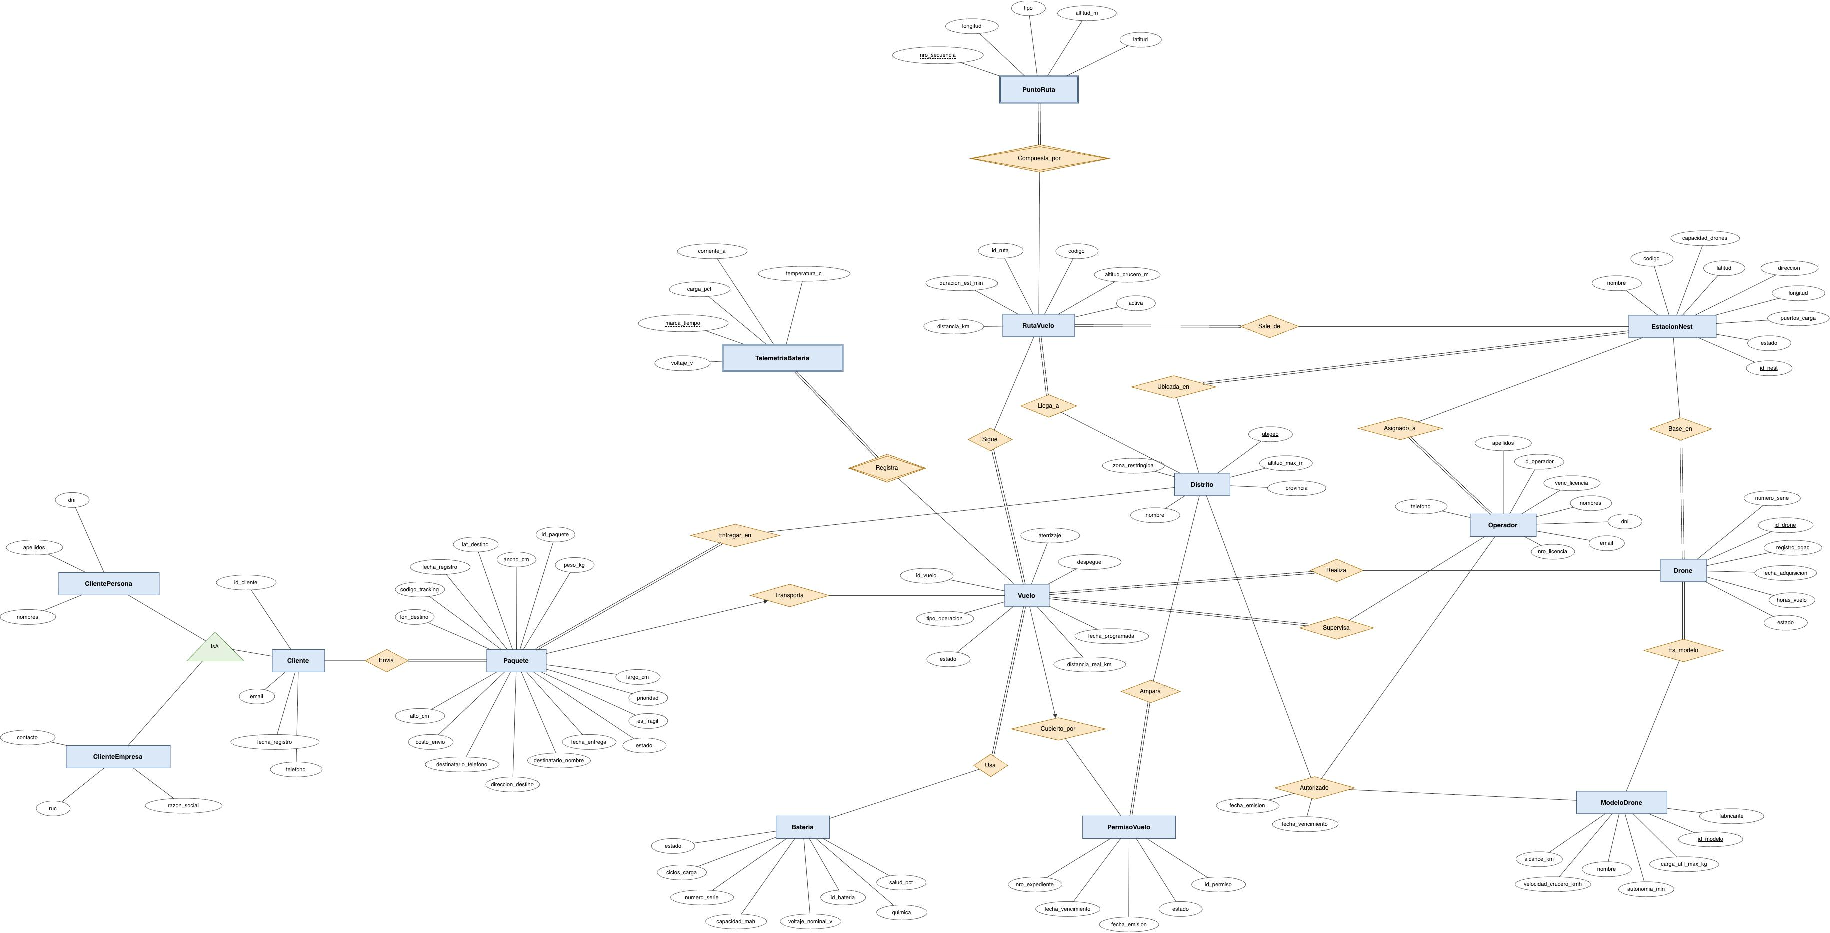
\includegraphics[width=\linewidth,height=0.9\textheight,keepaspectratio]{er.pdf}
\caption{Modelo Entidad-Relación de SkyNest (notación de Ramakrishnan y Gehrke).}
\label{fig:er}
\end{figure}
\end{landscape}}

\subsection{Especificaciones y consideraciones sobre el modelo}
El modelo tiene 15 conjuntos de entidades: 11 fuertes, 2 subclases y 2 débiles. Las cinco tablas exigidas por el tópico corresponden a \textit{Drone}, \textit{EstacionNest}, \textit{RutaVuelo}, \textit{Paquete} y \textit{TelemetriaBateria}. A continuación se detalla cada uno.

\subsubsection{Entidad Distrito}
\textbf{Especificaciones:} Representa cada distrito de Lima Metropolitana y el Callao. Su clave es \at{ubigeo}, el código oficial del INEI, y sus atributos descriptivos son \at{nombre}, \at{provincia}, \at{zona\_restringida} y \at{altitud\_max\_m}.

\textbf{Consideraciones:} Se eligió \at{ubigeo} como clave en lugar de una clave sustituta porque es un código oficial, estable y de solo 6 caracteres, y porque permitirá cruzar los datos con fuentes públicas del INEI. El distrito es el eje geográfico del modelo: de él dependen las restricciones de espacio aéreo, el destino de las rutas y el destino de los paquetes.

\subsubsection{Entidad EstacionNest}
\textbf{Especificaciones:} Almacena cada base física de despegue y aterrizaje: \at{codigo}, \at{nombre}, \at{direccion}, coordenadas, \at{capacidad\_drones}, \at{puertos\_carga} y \at{estado}. Su clave es la clave sustituta \at{id\_nest}.

\textbf{Consideraciones:} Se usa clave sustituta porque el código operativo puede cambiar si la empresa reorganiza su nomenclatura; el código se conserva como clave candidata. La participación en \textit{Ubicada\_en} es total: no tiene sentido un nest sin distrito.

\subsubsection{Entidad ModeloDrone}
\textbf{Especificaciones:} Guarda las características técnicas de cada modelo de aeronave: \at{fabricante}, \at{nombre}, \at{carga\_util\_max\_kg}, \at{autonomia\_min}, \at{velocidad\_crucero\_kmh} y \at{alcance\_km}.

\textbf{Consideraciones:} Se separó del drone para no repetir las mismas características técnicas en cada una de las 300 aeronaves, que es la redundancia que advierte el libro en el ap.~2.5.2. La clave candidata natural es el par (\at{fabricante}, \at{nombre}); se conserva como \texttt{UNIQUE}.

\subsubsection{Entidad Drone}
\textbf{Especificaciones:} Representa cada aeronave física: \at{numero\_serie}, \at{registro\_dgac}, \at{fecha\_adquisicion}, \at{estado} y \at{horas\_vuelo}.

\textbf{Consideraciones:} Tiene dos claves candidatas naturales, el número de serie del fabricante y el código de registro ante la DGAC, ambas declaradas \texttt{UNIQUE}. El atributo \at{horas\_vuelo} sí se almacena, aunque podría derivarse de los vuelos, porque incluye horas previas a la puesta en marcha del sistema y porque se consulta en cada programación de vuelo; se mantendrá actualizado con un trigger.

\subsubsection{Entidad Bateria}
\textbf{Especificaciones:} Registra cada batería intercambiable: \at{numero\_serie}, \at{quimica}, \at{capacidad\_mah}, \at{voltaje\_nominal\_v}, \at{ciclos\_carga}, \at{salud\_pct} y \at{estado}.

\textbf{Consideraciones:} Se modela como entidad propia y no como atributo del drone porque las baterías se intercambian entre aeronaves y porque su degradación es el dato central del mantenimiento preventivo. La batería que usa cada vuelo se captura con la relación \textit{Usa}, de modo que el historial de uso se obtiene consultando los vuelos.

\subsubsection{Entidad Operador}
\textbf{Especificaciones:} Guarda al piloto RPAS: \at{dni}, \at{nombres}, \at{apellidos}, \at{email}, \at{telefono}, \at{nro\_licencia} y \at{venc\_licencia}.

\textbf{Consideraciones:} Tiene tres claves candidatas naturales (DNI, email y número de licencia). Participa de forma total en \textit{Asignado\_a}, porque todo operador pertenece a un nest, y de forma parcial en \textit{Autorizado}, porque un operador recién contratado puede no tener autorizaciones todavía.

\subsubsection{Entidad Cliente}
\textbf{Especificaciones:} Superclase con los datos comunes de quien envía paquetes: \at{email}, \at{telefono} y \at{fecha\_registro}.

\textbf{Consideraciones:} Se especializa en \textit{ClientePersona} y \textit{ClienteEmpresa} porque los atributos identificatorios son excluyentes. Se declara la cobertura (\textsc{cubren}) y, al no declararse \textsc{solapa a}, las subclases no se solapan. Se mantiene la superclase porque \textit{Paquete} necesita relacionarse con cualquier cliente sin importar su tipo.

\subsubsection{Entidad ClientePersona}
\textbf{Especificaciones:} Subclase con \at{dni}, \at{nombres} y \at{apellidos}.

\textbf{Consideraciones:} Hereda la clave \at{id\_cliente} de la superclase. El DNI es clave candidata dentro de la subclase, no de \textit{Cliente}, porque una empresa no tiene DNI.

\subsubsection{Entidad ClienteEmpresa}
\textbf{Especificaciones:} Subclase con \at{ruc}, \at{razon\_social} y \at{contacto}.

\textbf{Consideraciones:} Hereda la clave de la superclase. El RUC es clave candidata dentro de la subclase. Este desdoblamiento permite declarar ambos campos obligatorios en su propia tabla, en lugar de dejarlos nulos en una tabla única.

\subsubsection{Entidad Paquete}
\textbf{Especificaciones:} Es el objeto que se transporta: \at{codigo\_tracking}, peso y dimensiones, \at{prioridad}, \at{es\_fragil}, datos del destinatario, dirección y coordenadas de entrega, \at{estado}, fechas y \at{costo\_envio}.

\textbf{Consideraciones:} El código de tracking es clave candidata, pero la clave principal es sustituta porque la tabla llegará al millón de registros y se relaciona con la telemetría y los vuelos. La participación en \textit{Transporta} es parcial en ambos lados: un paquete recién registrado aún no tiene vuelo, y un vuelo de retorno o de prueba no lleva paquetes. Los atributos de dimensiones y de destinatario se escribieron ya descompuestos, para que la traducción al modelo relacional sea directa.

\subsubsection{Entidad RutaVuelo}
\textbf{Especificaciones:} Corredor aéreo aprobado: \at{codigo}, \at{distancia\_km}, \at{altitud\_crucero\_m}, \at{duracion\_est\_min} y \at{activa}.

\textbf{Consideraciones:} Una ruta sale de un nest y llega a un distrito, y ambas participaciones son totales. Puede haber varias rutas entre el mismo nest y el mismo distrito (corredores distintos), por lo que el par (origen, destino) no es clave: por eso la distancia y la duración dependen de la ruta y no de ese par, lo que evita una violación de la FNBC.

\subsubsection{Entidad PuntoRuta}
\textbf{Especificaciones:} Entidad débil que representa cada waypoint de una ruta: \at{latitud}, \at{longitud}, \at{altitud\_m} y \at{tipo}. Su clave parcial es \at{nro\_secuencia}.

\textbf{Consideraciones:} Cumple las dos condiciones del ap.~2.4.3: participa en una relación identificadora binaria de uno a varios con \textit{RutaVuelo} y su participación es total. Un mismo número de secuencia puede repetirse en rutas distintas, por lo que solo identifica dentro de su ruta. Se modela como entidad y no como atributo multivaluado porque cada punto tiene varios atributos propios y un orden.

\subsubsection{Entidad Vuelo}
\textbf{Especificaciones:} Ejecución concreta de una ruta: \at{fecha\_programada}, \at{despegue}, \at{aterrizaje}, \at{estado} y \at{distancia\_real\_km}.

\textbf{Consideraciones:} Es el centro del modelo: vincula drone, batería, ruta y operador, y a su vez es propietaria de la telemetría y transporta paquetes. No se almacena el peso total transportado, que se obtiene sumando los paquetes del vuelo, ni el nest de origen, que se obtiene de la ruta.

\subsubsection{Entidad PermisoVuelo}
\textbf{Especificaciones:} Representa el permiso que la autoridad aeronáutica otorga para operar sobre un distrito, con \at{nro\_expediente}, \at{fecha\_emision}, \at{fecha\_vencimiento} y \at{estado}. Su clave es \at{id\_permiso} y el número de expediente es clave candidata.

\textbf{Consideraciones:} Se modela como conjunto de entidades y no como atributo de Vuelo por dos razones: el permiso tiene identidad y vigencia propias, independientes de cualquier vuelo, y un mismo permiso puede cubrir varios vuelos hacia el mismo distrito, de modo que guardarlo en Vuelo repetiría el número y las fechas en cada fila. Su participación en \textit{Ampara} es total, porque todo permiso se emite para un distrito.

\subsubsection{Entidad TelemetriaBateria}
\textbf{Especificaciones:} Entidad débil con las lecturas periódicas de la batería durante un vuelo: \at{voltaje\_v}, \at{corriente\_a}, \at{temperatura\_c} y \at{carga\_pct}. Su clave parcial es \at{marca\_tiempo}.

\textbf{Consideraciones:} Su propietaria identificadora es \textit{Vuelo}, con participación total. Dos vuelos distintos pueden tener lecturas con la misma marca de tiempo, de modo que esta solo identifica dentro del vuelo. Es la tabla de mayor volumen del sistema y la que determinará el diseño de índices del Hito 2.

\subsubsection{Conjuntos de relaciones}
La Tabla~\ref{tab:rel} resume los 18 conjuntos de relaciones y la jerarquía de clases. En la columna ``Restricción de clave'' se indica la entidad desde la que sale la flecha, es decir, la que participa como máximo en una relación; en ``Participación total'', la entidad unida por doble línea.

\begin{table}[H]
\centering\small
\caption{Conjuntos de relaciones del modelo E/R y sus restricciones.}
\label{tab:rel}
\begin{tabularx}{\textwidth}{l l l X}
\toprule
Relación & Entidades & Restricción de clave & Participación total \\
\midrule
Ubicada\_en & EstacionNest -- Distrito & EstacionNest & EstacionNest \\
Es\_modelo & Drone -- ModeloDrone & Drone & Drone \\
Base\_en & Drone -- EstacionNest & Drone & Drone \\
Asignado\_a & Operador -- EstacionNest & Operador & Operador \\
Autorizado (ternaria) & Operador -- ModeloDrone -- Distrito & Ninguna & Ninguna \\
Sale\_de & RutaVuelo -- EstacionNest & RutaVuelo & RutaVuelo \\
Llega\_a & RutaVuelo -- Distrito & RutaVuelo & RutaVuelo \\
Compuesta\_por (identif.) & PuntoRuta -- RutaVuelo & PuntoRuta & PuntoRuta \\
Realiza & Vuelo -- Drone & Vuelo & Vuelo \\
Usa & Vuelo -- Bateria & Vuelo & Vuelo \\
Sigue & Vuelo -- RutaVuelo & Vuelo & Vuelo \\
Supervisa & Vuelo -- Operador & Vuelo & Vuelo \\
Transporta & Paquete -- Vuelo & Paquete & Ninguna \\
Envia & Paquete -- Cliente & Paquete & Paquete \\
Entregar\_en & Paquete -- Distrito & Paquete & Paquete \\
Registra (identif.) & TelemetriaBateria -- Vuelo & TelemetriaBateria & TelemetriaBateria \\
Ampara & PermisoVuelo -- Distrito & PermisoVuelo & PermisoVuelo \\
Cubierto\_por & Vuelo -- PermisoVuelo & Vuelo & Ninguna \\
\midrule
IsA & Cliente $\supset$ Persona, Empresa & Sin solapamiento & Cobertura total (\textsc{cubren}) \\
\bottomrule
\end{tabularx}
\end{table}

\subsubsection{Consideraciones generales de diseño}
\begin{itemize}
\item \textbf{Vuelo como conjunto de entidades y no como relación.} Un vuelo vincula un drone, una batería, una ruta y un operador, por lo que podría pensarse como una relación entre ellos. Pero en el modelo ER cada relación debe quedar identificada de manera unívoca por sus entidades participantes (Ramakrishnan y Gehrke, ap.~2.3), y un mismo drone puede repetir la misma ruta, con la misma batería y el mismo operador, muchas veces. Además, un vuelo tiene atributos propios y participa en otras relaciones (\textit{Transporta} y \textit{Registra}). Por eso se modela como conjunto de entidades, igual que el libro introduce un conjunto de entidades cuando una relación necesitaría repetirse (ap.~2.5.1).
\item \textbf{Autorizado como relación ternaria.} Siguiendo el criterio del ejemplo \textit{Contratos} del libro (ap.~2.5.3), la autorización asocia de manera inherente tres entidades. Tres relaciones binarias (operador--modelo, operador--distrito y modelo--distrito) no la expresan: que el operador pueda volar el modelo $M$ y pueda volar en el distrito $D$ no implica que esté autorizado para volar $M$ en $D$. Tampoco podrían representar los atributos \at{fecha\_emision} y \at{fecha\_vencimiento} de cada autorización. Cada terna aparece a lo sumo una vez, por lo que la relación queda identificada por sus participantes; al renovarse, se actualizan sus fechas.
\item \textbf{Una batería por vuelo.} Se asume que cada drone usa una sola batería (o pack) por vuelo. Así, la batería de cada lectura de telemetría queda determinada por el vuelo y no hace falta una segunda propietaria identificadora, lo que el libro no admite, porque la relación identificadora debe ser binaria (ap.~2.5.3).
\item \textbf{Posición fuera de la telemetría de batería.} La posición del drone (latitud, longitud y altitud) no describe a la batería. Se deja fuera de \textit{TelemetriaBateria} y del alcance del proyecto.
\item \textbf{Tipo de operación del vuelo.} El atributo \at{tipo\_operacion} de \textit{Vuelo} distingue el vuelo \at{manual}, pilotado de forma remota, del \at{automatico}, que ejecuta el plan de vuelo cargado. El plan de vuelo en sí no es un atributo: es la secuencia ordenada de \textit{PuntoRuta} de la ruta que sigue el vuelo.
\item \textbf{Datos que no se almacenan como atributos.} El peso total de un vuelo se calcula sumando los pesos de sus paquetes, y el historial de uso de una batería se obtiene de los vuelos que la usan. Guardarlos repetiría información, que es lo que el libro advierte en el ap.~2.5.2; se expondrán mediante vistas en el Hito 2.
\end{itemize}

% ================================================================ 3
\section{Modelo Relacional}

\subsection{Modelo Relacional}
Notación: \pk{subrayado} = clave principal; \fk{cursiva} = clave externa; UQ = clave candidata.

\begin{enumerate}[leftmargin=*, label=\arabic*.]
\item \tb{distrito}(\pk{ubigeo}, nombre, provincia, zona\_restringida, altitud\_max\_m)

\item \tb{estacion\_nest}(\pk{id\_nest}, codigo, nombre, direccion, latitud, longitud, capacidad\_drones, puertos\_carga, estado, \fk{ubigeo})\\
UQ(codigo); ubigeo $\rightarrow$ distrito

\item \tb{modelo\_drone}(\pk{id\_modelo}, fabricante, nombre, carga\_util\_max\_kg, autonomia\_min, velocidad\_crucero\_kmh, alcance\_km)\\
UQ(fabricante, nombre)

\item \tb{drone}(\pk{id\_drone}, numero\_serie, registro\_dgac, fecha\_adquisicion, estado, horas\_vuelo, \fk{id\_modelo}, \fk{id\_nest\_base})\\
UQ(numero\_serie); UQ(registro\_dgac); id\_modelo $\rightarrow$ modelo\_drone; id\_nest\_base $\rightarrow$ estacion\_nest

\item \tb{bateria}(\pk{id\_bateria}, numero\_serie, quimica, capacidad\_mah, voltaje\_nominal\_v, ciclos\_carga, salud\_pct, estado)\\
UQ(numero\_serie)

\item \tb{operador}(\pk{id\_operador}, dni, nombres, apellidos, email, telefono, nro\_licencia, venc\_licencia, \fk{id\_nest})\\
UQ(dni); UQ(email); UQ(nro\_licencia); id\_nest $\rightarrow$ estacion\_nest

\item \tb{autorizacion}(\pkfk{id\_operador}, \pkfk{id\_modelo}, \pkfk{ubigeo}, fecha\_emision, fecha\_vencimiento)\\
id\_operador $\rightarrow$ operador; id\_modelo $\rightarrow$ modelo\_drone; ubigeo $\rightarrow$ distrito

\item \tb{cliente}(\pk{id\_cliente}, email, telefono, fecha\_registro)\\
UQ(email)

\item \tb{cliente\_persona}(\pkfk{id\_cliente}, dni, nombres, apellidos)\\
UQ(dni); id\_cliente $\rightarrow$ cliente (ON DELETE CASCADE)

\item \tb{cliente\_empresa}(\pkfk{id\_cliente}, ruc, razon\_social, contacto)\\
UQ(ruc); id\_cliente $\rightarrow$ cliente (ON DELETE CASCADE)

\item \tb{ruta\_vuelo}(\pk{id\_ruta}, codigo, \fk{id\_nest\_origen}, \fk{ubigeo\_destino}, distancia\_km, altitud\_crucero\_m, duracion\_est\_min, activa)\\
UQ(codigo); id\_nest\_origen $\rightarrow$ estacion\_nest; ubigeo\_destino $\rightarrow$ distrito

\item \tb{punto\_ruta}(\pkfk{id\_ruta}, \pk{nro\_secuencia}, latitud, longitud, altitud\_m, tipo)\\
id\_ruta $\rightarrow$ ruta\_vuelo (ON DELETE CASCADE)

\item \tb{permiso\_vuelo}(\pk{id\_permiso}, nro\_expediente, \fk{ubigeo}, fecha\_emision, fecha\_vencimiento, estado)\\
UQ(nro\_expediente); ubigeo $\rightarrow$ distrito

\item \tb{vuelo}(\pk{id\_vuelo}, \fk{id\_drone}, \fk{id\_bateria}, \fk{id\_ruta}, \fk{id\_operador}, \fk{id\_permiso}, fecha\_programada, despegue, aterrizaje, estado, tipo\_operacion, distancia\_real\_km)\\
id\_drone $\rightarrow$ drone; id\_bateria $\rightarrow$ bateria; id\_ruta $\rightarrow$ ruta\_vuelo; id\_operador $\rightarrow$ operador; id\_permiso $\rightarrow$ permiso\_vuelo (admite NULL)

\item \tb{paquete}(\pk{id\_paquete}, codigo\_tracking, \fk{id\_cliente}, \fk{id\_vuelo}, \fk{ubigeo\_destino}, peso\_kg, largo\_cm, ancho\_cm, alto\_cm, prioridad, es\_fragil, destinatario\_nombre, destinatario\_telefono, direccion\_destino, lat\_destino, lon\_destino, estado, fecha\_registro, fecha\_entrega, costo\_envio)\\
UQ(codigo\_tracking); id\_cliente $\rightarrow$ cliente; id\_vuelo $\rightarrow$ vuelo (admite NULL); ubigeo\_destino $\rightarrow$ distrito

\item \tb{telemetria\_bateria}(\pkfk{id\_vuelo}, \pk{marca\_tiempo}, voltaje\_v, corriente\_a, temperatura\_c, carga\_pct)\\
id\_vuelo $\rightarrow$ vuelo (ON DELETE CASCADE)
\end{enumerate}

\paragraph{Normalización.} Todas las relaciones están en \textbf{forma normal de Boyce-Codd (FNBC)} y, por tanto, en 3FN:
\begin{itemize}
\item \textbf{1FN}: todos los atributos son atómicos y no hay atributos multivaluados; los puntos de una ruta se separaron en \tb{punto\_ruta}.
\item \textbf{2FN}: en las tablas con clave compuesta (\tb{autorizacion}, \tb{punto\_ruta} y \tb{telemetria\_bateria}), cada atributo no clave depende de la clave completa. Por ejemplo, las fechas de una autorización dependen de la terna completa (operador, modelo, distrito), y las mediciones de una lectura dependen del par (vuelo, marca de tiempo).
\item \textbf{3FN/FNBC}: los únicos determinantes de cada tabla son sus claves candidatas. Por ejemplo, en \tb{paquete} los datos del cliente no se repiten, sino que se obtienen mediante \at{id\_cliente}. En \tb{vuelo}, el nest de origen no se almacena porque se deriva de la ruta. En \tb{drone}, las características técnicas están en \tb{modelo\_drone}. En \tb{ruta\_vuelo}, la distancia depende de la ruta y no del par (origen, destino), porque puede haber varios corredores entre el mismo nest y el mismo distrito. En \tb{telemetria\_bateria} no se guarda \at{id\_bateria}: dependería de \at{id\_vuelo} (dependencia transitiva), así que la batería se obtiene del vuelo.
\end{itemize}

\paragraph{Restricciones de integridad adicionales.} Varias reglas semánticas no se pueden expresar con claves ni con claves externas; el libro indica que requieren restricciones de tabla o asertos (ap.~3.5.4 y 3.5.6). Como PostgreSQL no implementa \texttt{CREATE ASSERTION}, se implementarán en el Hito 2 con triggers y restricciones \texttt{CHECK}:
\begin{enumerate}[label=(\roman*)]
\item cobertura y no solapamiento de la jerarquía de clientes;
\item peso total por vuelo $\leq$ carga útil del modelo;
\item licencia vigente y autorización vigente del operador para el modelo y el distrito;
\item permiso vigente para todo vuelo cuya ruta llegue a un distrito restringido;
\item coincidencia entre el distrito de entrega del paquete y el distrito al que llega la ruta;
\item nest base del drone igual al nest de salida de la ruta;
\item no solapamiento de vuelos que usan la misma batería, mediante una restricción \texttt{EXCLUDE} con \texttt{btree\_gist};
\item marca de tiempo de la telemetría dentro del intervalo del vuelo;
\item capacidad del nest no excedida;
\item al menos dos puntos por ruta.
\end{enumerate}

\subsection{Especificaciones de transformación}
La traducción sigue el procedimiento del apartado 3.5 de Ramakrishnan y Gehrke.

\subsubsection{Entidades}
Cada conjunto de entidades fuerte se tradujo a una tabla cuyos campos son sus atributos y cuya clave principal es la clave del conjunto (ap.~3.5.1). En las entidades cuyos identificadores naturales pueden cambiar o son largos, se usó una clave sustituta entera (\at{id\_*}, tipo \texttt{SERIAL}: entero de 4 bytes que PostgreSQL numera automáticamente y admite hasta unos 2\,100 millones de valores, holgado para el volumen estimado), y las claves naturales se conservaron como claves candidatas (\texttt{UNIQUE}), por ejemplo \at{numero\_serie}, \at{codigo\_tracking} o \at{dni}. En \tb{distrito} se usó como clave principal el código natural \at{ubigeo}, que es estable y oficial.

\subsubsection{Entidades débiles}
Según el ap.~3.5.5, cada conjunto de entidades débiles se tradujo junto con su relación identificadora a una sola tabla. La clave principal es la clave parcial más la clave de la propietaria identificadora, y la clave externa usa \texttt{ON DELETE CASCADE} para que las entidades débiles se eliminen junto con su propietaria:
\begin{itemize}
\item \textbf{PuntoRuta} + \textit{Compuesta\_por} $\rightarrow$ \tb{punto\_ruta}, con clave principal (\at{id\_ruta}, \at{nro\_secuencia}).
\item \textbf{TelemetriaBateria} + \textit{Registra} $\rightarrow$ \tb{telemetria\_bateria}, con clave principal (\at{id\_vuelo}, \at{marca\_tiempo}).
\end{itemize}
En ambos casos la participación total queda garantizada porque la clave externa forma parte de la clave principal, lo que la hace implícitamente \texttt{NOT NULL}.

\subsubsection{Entidades superclase/subclases}
La jerarquía \textit{Cliente} $\supset$ \{\textit{ClientePersona}, \textit{ClienteEmpresa}\} se tradujo con el \textbf{primer enfoque} del ap.~3.5.6: una tabla por cada conjunto de entidades. \tb{cliente} guarda los atributos comunes y cada subclase tiene su tabla, cuya clave principal (\at{id\_cliente}) es a la vez clave externa hacia \tb{cliente}, con eliminación en cascada.

Se descartó el segundo enfoque (una tabla por subclase sin superclase) por dos razones. La primera es que \tb{paquete} necesita una única clave externa hacia ``el cliente'', sin importar su tipo. La segunda es que muchas consultas examinan a todos los clientes, y el libro señala que el primer enfoque las facilita. Como indica el libro, las restricciones de cobertura y de solapamiento solo pueden expresarse con asertos, por lo que se implementarán con triggers.

\subsubsection{Relaciones binarias}
Todas las relaciones binarias del modelo tienen restricción de clave en uno de sus lados, así que ninguna genera tabla propia. Se tradujeron con el \textbf{segundo enfoque} del ap.~3.5.3: la clave de la otra entidad se añade como clave externa a la tabla de la entidad con restricción de clave. El libro recomienda este enfoque, sobre todo cuando además hay participación total (ap.~3.5.4). Cuando la participación es total, la clave externa se declara \texttt{NOT NULL} con \texttt{ON DELETE NO ACTION}, de modo que no se pueda borrar, por ejemplo, un drone que ya tiene vuelos registrados.

\begin{enumerate}[leftmargin=*]
\item \textbf{Ubicada\_en} (EstacionNest--Distrito, de una a varias, total en EstacionNest): \at{ubigeo} pasa a \tb{estacion\_nest} como clave externa \texttt{NOT NULL}.
\item \textbf{Es\_modelo} (Drone--ModeloDrone, de una a varias, total en Drone): \at{id\_modelo} pasa a \tb{drone} como clave externa \texttt{NOT NULL}.
\item \textbf{Base\_en} (Drone--EstacionNest, de una a varias, total en Drone): \at{id\_nest\_base} pasa a \tb{drone} como clave externa \texttt{NOT NULL}.
\item \textbf{Asignado\_a} (Operador--EstacionNest, de una a varias, total en Operador): \at{id\_nest} pasa a \tb{operador} como clave externa \texttt{NOT NULL}.
\item \textbf{Sale\_de} (RutaVuelo--EstacionNest, de una a varias, total en RutaVuelo): \at{id\_nest\_origen} pasa a \tb{ruta\_vuelo} como clave externa \texttt{NOT NULL}.
\item \textbf{Llega\_a} (RutaVuelo--Distrito, de una a varias, total en RutaVuelo): \at{ubigeo\_destino} pasa a \tb{ruta\_vuelo} como clave externa \texttt{NOT NULL}.
\item \textbf{Realiza}, \textbf{Usa}, \textbf{Sigue} y \textbf{Supervisa} (Vuelo con Drone, Bateria, RutaVuelo y Operador; todas de una a varias y totales en Vuelo): las cuatro claves pasan a \tb{vuelo} como claves externas \texttt{NOT NULL}.
\item \textbf{Envia} (Paquete--Cliente, de una a varias, total en Paquete): \at{id\_cliente} pasa a \tb{paquete} como clave externa \texttt{NOT NULL}.
\item \textbf{Entregar\_en} (Paquete--Distrito, de una a varias, total en Paquete): \at{ubigeo\_destino} pasa a \tb{paquete} como clave externa \texttt{NOT NULL}.
\item \textbf{Ampara} (PermisoVuelo--Distrito, de una a varias, total en PermisoVuelo): \at{ubigeo} pasa a \tb{permiso\_vuelo} como clave externa \texttt{NOT NULL}.
\item \textbf{Cubierto\_por} (Vuelo--PermisoVuelo, con restricción de clave en Vuelo y participación parcial en ambos lados): \at{id\_permiso} pasa a \tb{vuelo} como clave externa que \textbf{admite NULL}, porque los vuelos hacia distritos sin restricción no requieren permiso.
\item \textbf{Transporta} (Paquete--Vuelo, de una a varias, con restricción de clave en Paquete y participación parcial en ambos lados): \at{id\_vuelo} pasa a \tb{paquete} como clave externa que \textbf{admite NULL} mientras el paquete no tenga vuelo asignado. El libro advierte que este enfoque puede dejar valores nulos (ap.~3.5.3); se aceptan porque evitan una tabla adicional y una combinación de dos tablas en la consulta más frecuente, el seguimiento de un paquete.
\item \textbf{Compuesta\_por} y \textbf{Registra} son relaciones identificadoras y ya se trataron en el apartado de entidades débiles: no generan tabla propia, sino que se absorben en \tb{punto\_ruta} y \tb{telemetria\_bateria}.
\end{enumerate}

No hay relaciones binarias de varias a varias en el modelo, por lo que ninguna relación binaria requirió tabla propia.

\subsubsection{Relaciones ternarias}\label{sec:ternaria}
La relación ternaria \textbf{Autorizado} (Operador, ModeloDrone, Distrito) no tiene restricciones de clave ni de participación. Se tradujo como indica el ap.~3.5.2 (ejemplo \textit{Trabaja\_en2}) a la tabla \tb{autorizacion}. Sus campos son las claves principales de los tres conjuntos de entidades participantes, cada una declarada como clave externa, más los atributos descriptivos \at{fecha\_emision} y \at{fecha\_vencimiento}. Como no hay restricciones de clave, el conjunto de las tres claves externas (\at{id\_operador}, \at{id\_modelo}, \at{ubigeo}) es clave candidata y se elige como clave principal, lo que hace implícitamente \texttt{NOT NULL} cada uno de esos campos.

\subsection{Diccionario de datos}
{\small
\setlength{\tabcolsep}{4pt}
\newcommand{\dict}[1]{%
\par\noindent\textbf{Tabla \texttt{#1}}\par\nopagebreak}
\newenvironment{dtab}{%
\begin{longtable}{>{\ttfamily\raggedright\arraybackslash}p{3.3cm} >{\raggedright\arraybackslash}p{2.5cm} c >{\raggedright\arraybackslash}p{3.6cm} >{\raggedright\arraybackslash}p{4.3cm}}
\toprule
\normalfont\textbf{Atributo} & \textbf{Tipo} & \textbf{Nulo} & \textbf{Restricciones} & \textbf{Descripción}\\
\midrule\endhead}{\bottomrule\end{longtable}}

\dict{distrito}
\begin{dtab}
ubigeo & CHAR(6) & No & PK; solo dígitos & Código UBIGEO del INEI \\
nombre & VARCHAR(60) & No & & Nombre del distrito \\
provincia & VARCHAR(30) & No & IN ('Lima', 'Callao') & Provincia \\
zona\_restringida & BOOLEAN & No & DEFAULT FALSE & Espacio aéreo restringido \\
altitud\_max\_m & NUMERIC(5,1) & No & $> 0$; DEFAULT 120 & Altitud máxima de vuelo permitida (m) \\
\end{dtab}

\dict{estacion\_nest}
\begin{dtab}
id\_nest & SERIAL & No & PK & Identificador del nest \\
codigo & VARCHAR(12) & No & UNIQUE & Código operativo (p.\,ej. NST-MIR-01) \\
nombre & VARCHAR(80) & No & & Nombre de la estación \\
direccion & VARCHAR(150) & No & & Dirección física \\
latitud & NUMERIC(9,6) & No & $[-90,90]$ & Latitud \\
longitud & NUMERIC(9,6) & No & $[-180,180]$ & Longitud \\
capacidad\_drones & SMALLINT & No & $> 0$ & Máximo de drones con base aquí \\
puertos\_carga & SMALLINT & No & $\geq 0$ & Número de puertos de carga \\
estado & VARCHAR(15) & No & IN ('operativa', 'mantenimiento', 'inactiva') & Estado del nest \\
ubigeo & CHAR(6) & No & FK $\rightarrow$ distrito & Distrito donde se ubica \\
\end{dtab}

\dict{modelo\_drone}
\begin{dtab}
id\_modelo & SERIAL & No & PK & Identificador del modelo \\
fabricante & VARCHAR(50) & No & UNIQUE(fabricante, nombre) & Fabricante \\
nombre & VARCHAR(50) & No & & Nombre comercial \\
carga\_util\_max\_kg & NUMERIC(5,2) & No & $> 0$ & Carga útil máxima (kg) \\
autonomia\_min & SMALLINT & No & $> 0$ & Autonomía con carga (min) \\
velocidad\_crucero\_kmh & NUMERIC(5,1) & No & $> 0$ & Velocidad de crucero (km/h) \\
alcance\_km & NUMERIC(5,1) & No & $> 0$ & Alcance máximo (km) \\
\end{dtab}

\dict{drone}
\begin{dtab}
id\_drone & SERIAL & No & PK & Identificador del drone \\
numero\_serie & VARCHAR(30) & No & UNIQUE & Número de serie del fabricante \\
registro\_dgac & VARCHAR(20) & No & UNIQUE & Código de registro RPAS ante la DGAC \\
fecha\_adquisicion & DATE & No & & Fecha de compra \\
estado & VARCHAR(15) & No & IN ('disponible', 'en\_vuelo', 'cargando', 'mantenimiento', 'baja') & Estado actual \\
horas\_vuelo & NUMERIC(8,2) & No & $\geq 0$; DEFAULT 0 & Horas de vuelo acumuladas \\
id\_modelo & INTEGER & No & FK $\rightarrow$ modelo\_drone & Modelo del drone \\
id\_nest\_base & INTEGER & No & FK $\rightarrow$ estacion\_nest & Nest base \\
\end{dtab}

\dict{bateria}
\begin{dtab}
id\_bateria & SERIAL & No & PK & Identificador de la batería \\
numero\_serie & VARCHAR(30) & No & UNIQUE & Número de serie \\
quimica & VARCHAR(10) & No & IN ('LiPo', 'Li-ion', 'LiHV') & Química de la celda \\
capacidad\_mah & INTEGER & No & $> 0$ & Capacidad nominal (mAh) \\
voltaje\_nominal\_v & NUMERIC(5,2) & No & $> 0$ & Voltaje nominal (V) \\
ciclos\_carga & INTEGER & No & $\geq 0$; DEFAULT 0 & Ciclos de carga acumulados \\
salud\_pct & NUMERIC(5,2) & No & $[0,100]$ & Estado de salud (SoH) \\
estado & VARCHAR(12) & No & IN ('operativa', 'degradada', 'baja') & Estado de la batería \\
\end{dtab}

\dict{operador}
\begin{dtab}
id\_operador & SERIAL & No & PK & Identificador del operador \\
dni & CHAR(8) & No & UNIQUE; 8 dígitos & DNI \\
nombres & VARCHAR(60) & No & & Nombres \\
apellidos & VARCHAR(60) & No & & Apellidos \\
email & VARCHAR(100) & No & UNIQUE & Correo electrónico \\
telefono & VARCHAR(15) & Sí & & Teléfono \\
nro\_licencia & VARCHAR(20) & No & UNIQUE & Licencia de piloto RPAS \\
venc\_licencia & DATE & No & & Vencimiento de la licencia \\
id\_nest & INTEGER & No & FK $\rightarrow$ estacion\_nest & Nest asignado \\
\end{dtab}

\dict{autorizacion}
\begin{dtab}
id\_operador & INTEGER & No & PK; FK $\rightarrow$ operador & Operador autorizado \\
id\_modelo & INTEGER & No & PK; FK $\rightarrow$ modelo\_drone & Modelo de drone autorizado \\
ubigeo & CHAR(6) & No & PK; FK $\rightarrow$ distrito & Distrito autorizado \\
fecha\_emision & DATE & No & & Fecha de emisión \\
fecha\_vencimiento & DATE & No & $>$ fecha\_emision & Fecha de vencimiento \\
\end{dtab}

\dict{cliente}
\begin{dtab}
id\_cliente & SERIAL & No & PK & Identificador del cliente \\
email & VARCHAR(100) & No & UNIQUE & Correo electrónico \\
telefono & VARCHAR(15) & Sí & & Teléfono \\
fecha\_registro & TIMESTAMP & No & DEFAULT now() & Fecha de alta \\
\end{dtab}

\dict{cliente\_persona}
\begin{dtab}
id\_cliente & INTEGER & No & PK; FK $\rightarrow$ cliente & Cliente persona natural \\
dni & CHAR(8) & No & UNIQUE; 8 dígitos & DNI \\
nombres & VARCHAR(60) & No & & Nombres \\
apellidos & VARCHAR(60) & No & & Apellidos \\
\end{dtab}

\dict{cliente\_empresa}
\begin{dtab}
id\_cliente & INTEGER & No & PK; FK $\rightarrow$ cliente & Cliente empresa \\
ruc & CHAR(11) & No & UNIQUE; 11 dígitos & RUC \\
razon\_social & VARCHAR(120) & No & & Razón social \\
contacto & VARCHAR(80) & Sí & & Persona de contacto \\
\end{dtab}

\dict{ruta\_vuelo}
\begin{dtab}
id\_ruta & SERIAL & No & PK & Identificador de la ruta \\
codigo & VARCHAR(15) & No & UNIQUE & Código de la ruta \\
id\_nest\_origen & INTEGER & No & FK $\rightarrow$ estacion\_nest & Nest del que sale \\
ubigeo\_destino & CHAR(6) & No & FK $\rightarrow$ distrito & Distrito al que llega \\
distancia\_km & NUMERIC(6,2) & No & $> 0$ & Distancia de la ruta (km) \\
altitud\_crucero\_m & NUMERIC(5,1) & No & $> 0$ & Altitud de crucero (m) \\
duracion\_est\_min & SMALLINT & No & $> 0$ & Duración estimada (min) \\
activa & BOOLEAN & No & DEFAULT TRUE & Ruta habilitada \\
\end{dtab}

\dict{punto\_ruta}
\begin{dtab}
id\_ruta & INTEGER & No & PK; FK $\rightarrow$ ruta\_vuelo & Ruta propietaria \\
nro\_secuencia & SMALLINT & No & PK; $\geq 1$ & Orden del punto en la ruta (clave parcial) \\
latitud & NUMERIC(9,6) & No & $[-90,90]$ & Latitud \\
longitud & NUMERIC(9,6) & No & $[-180,180]$ & Longitud \\
altitud\_m & NUMERIC(5,1) & No & $\geq 0$ & Altitud del punto (m) \\
tipo & VARCHAR(12) & No & IN ('despegue', 'paso', 'entrega', 'aterrizaje') & Tipo de punto \\
\end{dtab}

\dict{permiso\_vuelo}
\begin{dtab}
id\_permiso & SERIAL & No & PK & Identificador del permiso \\
nro\_expediente & VARCHAR(20) & No & UNIQUE & Número de expediente ante la autoridad \\
ubigeo & CHAR(6) & No & FK $\rightarrow$ distrito & Distrito que ampara el permiso \\
fecha\_emision & DATE & No & & Fecha de emisión \\
fecha\_vencimiento & DATE & No & $>$ fecha\_emision & Fecha de vencimiento \\
estado & VARCHAR(12) & No & IN ('vigente', 'vencido', 'revocado') & Estado del permiso \\
\end{dtab}

\dict{vuelo}
\begin{dtab}
id\_vuelo & SERIAL & No & PK & Identificador del vuelo \\
id\_drone & INTEGER & No & FK $\rightarrow$ drone & Drone que vuela \\
id\_bateria & INTEGER & No & FK $\rightarrow$ bateria & Batería usada \\
id\_ruta & INTEGER & No & FK $\rightarrow$ ruta\_vuelo & Ruta seguida \\
id\_operador & INTEGER & No & FK $\rightarrow$ operador & Operador supervisor \\
id\_permiso & INTEGER & Sí & FK $\rightarrow$ permiso\_vuelo & Permiso que ampara el vuelo \\
fecha\_programada & TIMESTAMP & No & & Hora programada de salida \\
despegue & TIMESTAMP & Sí & & Hora real de despegue \\
aterrizaje & TIMESTAMP & Sí & $>$ despegue & Hora real de aterrizaje \\
estado & VARCHAR(12) & No & IN ('programado', 'en\_curso', 'completado', 'abortado', 'cancelado') & Estado del vuelo \\
tipo\_operacion & VARCHAR(10) & No & IN ('manual', 'automatico') & Vuelo pilotado o por plan de vuelo \\
distancia\_real\_km & NUMERIC(6,2) & Sí & $> 0$ & Distancia realmente recorrida \\
\end{dtab}

\dict{paquete}
\begin{dtab}
id\_paquete & SERIAL & No & PK & Identificador del paquete \\
codigo\_tracking & CHAR(12) & No & UNIQUE & Código de seguimiento \\
id\_cliente & INTEGER & No & FK $\rightarrow$ cliente & Cliente remitente \\
id\_vuelo & INTEGER & Sí & FK $\rightarrow$ vuelo & Vuelo que lo transporta \\
ubigeo\_destino & CHAR(6) & No & FK $\rightarrow$ distrito & Distrito de entrega \\
peso\_kg & NUMERIC(5,2) & No & $> 0$ & Peso (kg) \\
largo\_cm & NUMERIC(5,1) & No & $> 0$ & Largo (cm) \\
ancho\_cm & NUMERIC(5,1) & No & $> 0$ & Ancho (cm) \\
alto\_cm & NUMERIC(5,1) & No & $> 0$ & Alto (cm) \\
prioridad & VARCHAR(10) & No & IN ('estandar', 'express') & Nivel de servicio \\
es\_fragil & BOOLEAN & No & DEFAULT FALSE & Contenido frágil \\
destinatario\_nombre & VARCHAR(100) & No & & Nombre del destinatario \\
destinatario\_telefono & VARCHAR(15) & No & & Teléfono del destinatario \\
direccion\_destino & VARCHAR(150) & No & & Dirección de entrega \\
lat\_destino & NUMERIC(9,6) & Sí & $[-90,90]$ & Latitud de entrega \\
lon\_destino & NUMERIC(9,6) & Sí & $[-180,180]$ & Longitud de entrega \\
estado & VARCHAR(12) & No & IN ('registrado', 'asignado', 'en\_ruta', 'entregado', 'fallido', 'devuelto') & Estado del envío \\
fecha\_registro & TIMESTAMP & No & DEFAULT now() & Fecha de registro \\
fecha\_entrega & TIMESTAMP & Sí & $\geq$ fecha\_registro & Fecha y hora de entrega \\
costo\_envio & NUMERIC(8,2) & No & $\geq 0$ & Costo del envío (S/) \\
\end{dtab}

\dict{telemetria\_bateria}
\begin{dtab}
id\_vuelo & INTEGER & No & PK; FK $\rightarrow$ vuelo & Vuelo de la lectura (propietaria) \\
marca\_tiempo & TIMESTAMP(3) & No & PK & Instante de la lectura (clave parcial) \\
voltaje\_v & NUMERIC(5,2) & No & $> 0$ & Voltaje medido (V) \\
corriente\_a & NUMERIC(6,2) & No & & Corriente (A); negativa en regeneración \\
temperatura\_c & NUMERIC(5,2) & No & $[-20,90]$ & Temperatura de la batería (°C) \\
carga\_pct & NUMERIC(5,2) & No & $[0,100]$ & Estado de carga (SoC) \\
\end{dtab}
}



% ================================================================ HITO 2
% =====================================================================
% SkyNest · Hito 2: secciones 4 a 7
% Los resultados del experimento se leen de resultados/ (bench/experimento.py).
% Las cifras citadas en el texto corresponden a la corrida oficial del 14/11/2026
% (Apple M1, PostgreSQL 14.25) guardada en resultados/.
% =====================================================================

\newpage
\section{Implementación de la base de datos}

La base se implementó en PostgreSQL 14 con scripts SQL numerados que se ejecutan en orden. Todos se pueden volver a ejecutar sin errores y cada uno tiene un script de prueba que deja la base como estaba (transacción con \texttt{ROLLBACK}).

\begin{table}[H]
\centering\small
\caption{Scripts de la implementación}
\label{tab:scripts}
\begin{tabularx}{\linewidth}{@{}>{\raggedright\arraybackslash}p{5cm}>{\raggedright\arraybackslash}X@{}}
\toprule
Script & Contenido \\
\midrule
\archivo{sql/01_schema.sql} & esquemas \texttt{skynest} y \texttt{reportes}; 16 tablas con PK, FK, UNIQUE, CHECK y EXCLUDE (sección~\ref{sec:tablas}) \\
\archivo{sql/02_datos_reales.sql} & distritos, modelos de drone y nests reales (sección~\ref{sec:carga}) \\
\archivo{gen/generar.py} & generador de datos sintéticos coherentes y carga con \texttt{COPY} \\
\archivo{sql/03_triggers.sql} & 17 triggers: restricciones (i)--(x) y automatización de estados \\
\archivo{sql/04_procedimientos.sql} & 9 procedimientos del flujo de un envío \\
\archivo{sql/05_vistas.sql} & 9 vistas de usuario y la función de rastreo \\
\archivo{sql/06_roles.sql} & 7 roles con privilegios mínimos \\
\archivo{sql/07_consultas.sql}\newline\archivo{sql/08_indices.sql} & consultas y planes de índices del experimento \\
\archivo{gen/construir_bases.sh} & construye las 4 bases, las verifica y genera los 4 dumps \\
\archivo{bench/experimento.py} & ejecuta el experimento y genera tablas y gráficos \\
\bottomrule
\end{tabularx}
\end{table}

% ---------------------------------------------------------------------
\subsection{Creación de Tablas en PostgreSQL}
\label{sec:tablas}

\archivo{sql/01_schema.sql} traduce el diccionario de datos de la sección 3.3 sin cambios de nombres, tipos ni nulos, para que el modelo físico coincida con el relacional. Las decisiones de implementación fueron:

\begin{enumerate}[label=\arabic*.]
\item \textbf{Restricciones con nombre} (\texttt{pk\_}, \texttt{fk\_}, \texttt{uq\_}, \texttt{ck\_}, \texttt{ex\_}). Así, cada error indica qué regla se violó, por ejemplo \texttt{violates check constraint "ck\_telemetria\_carga"}.
\item \textbf{Las reglas que solo dependen de una fila se implementaron como CHECK}, no como trigger: los dominios de R18 y las dos condiciones de R19. Además se agregaron tres CHECK que implementan reglas ya existentes:
  \begin{itemize}
  \item \texttt{ck\_bateria\_salud\_estado}: una batería con \at{salud\_pct} $< 70$ no puede estar \at{operativa} (R12).
  \item \texttt{ck\_vuelo\_estado\_tiempos}: el estado del vuelo es coherente con sus horarios. Un vuelo \at{programado} o \at{cancelado} no tiene despegue; uno \at{completado} tiene despegue y aterrizaje.
  \item \texttt{ck\_paquete\_coordenadas}: la latitud y la longitud de destino se registran juntas o faltan juntas.
  \end{itemize}
\item \textbf{R12 (una batería no puede estar en dos vuelos a la vez) con una restricción \texttt{EXCLUDE}} sobre el par (batería, intervalo del vuelo), que requiere la extensión \texttt{btree\_gist}. Solo se aplica cuando el vuelo ya tiene despegue y aterrizaje:
\begin{lstlisting}[style=sql]
CONSTRAINT ex_vuelo_bateria_solape EXCLUDE USING gist (
    id_bateria WITH =,
    tsrange(despegue, aterrizaje) WITH &&
) WHERE (despegue IS NOT NULL AND aterrizaje IS NOT NULL)
\end{lstlisting}
\item \textbf{ON DELETE}: \texttt{CASCADE} en las entidades débiles (\tb{punto\_ruta}, \tb{telemetria\_bateria}) y en las subclases de cliente; en las demás FK, el valor por defecto (\texttt{NO ACTION}), que impide, por ejemplo, borrar un drone que ya voló.
\item \textbf{Sin índices adicionales}: solo existen los que PostgreSQL crea por sí mismo para PRIMARY KEY, UNIQUE y EXCLUDE. Las FOREIGN KEY no crean índice en PostgreSQL. Los índices del experimento se definen aparte (sección~\ref{sec:planes}).
\end{enumerate}

\archivo{sql/01_schema_prueba.sql} inserta un envío válido de punta a punta e intenta 13 violaciones (PK, UNIQUE, FK, CHECK y EXCLUDE). Las 13 son rechazadas con la restricción esperada.

% ---------------------------------------------------------------------
\subsubsection{Esquemas}
\label{sec:esquemas}

Un esquema es una carpeta con nombre dentro de la base: agrupa tablas, vistas y funciones, y se le pueden dar permisos como a un todo. La base \texttt{skynest\_<escala>} se organizó en dos esquemas:

\begin{table}[H]
\centering\small
\caption{Esquemas de la base}
\label{tab:esquemas}
\begin{tabular}{l>{\raggedright\arraybackslash}p{6.4cm}>{\raggedright\arraybackslash}p{5cm}}
\toprule
Esquema & Contenido & Quién entra (\texttt{USAGE}) \\
\midrule
\texttt{skynest} & el núcleo: 16 tablas, 12 funciones de trigger y 9 procedimientos & administrador, despachador, operador, técnico, telemetría y cliente \\
\texttt{reportes} & 9 vistas y la función de rastreo (\texttt{fn\_rastrear\_paquete}) & administrador, despachador, operador, técnico, analista y cliente \\
\texttt{public} & solo la extensión \texttt{btree\_gist} & --- \\
\bottomrule
\end{tabular}
\end{table}

La separación tiene dos efectos. Primero, el modelo queda ordenado: lo que se guarda (\texttt{skynest}) está aparte de lo que se consulta para reportar (\texttt{reportes}). Segundo, la seguridad es más simple: el analista recibe \texttt{USAGE} solo sobre \texttt{reportes}, por lo que no puede ni ver los nombres de las tablas del núcleo; si intenta \texttt{SELECT * FROM skynest.paquete}, PostgreSQL responde \texttt{permission denied for schema skynest} antes de revisar permisos de tabla.

Para no escribir el esquema en cada consulta, \archivo{sql/01_schema.sql} fija la ruta de búsqueda por defecto de la base:
\begin{lstlisting}[style=sql]
CREATE SCHEMA skynest;
CREATE SCHEMA reportes;
ALTER DATABASE skynest_1m SET search_path = skynest, reportes, public;
\end{lstlisting}
Así, \texttt{SELECT * FROM vuelo} se resuelve como \texttt{skynest.vuelo} y \texttt{v\_peso\_vuelo} como \texttt{reportes.v\_peso\_vuelo}. Los procedimientos \texttt{SECURITY DEFINER} y la función de rastreo fijan su propio \texttt{search\_path}, para que un usuario no pueda engañarlos creando una tabla con el mismo nombre en otro esquema.

% ---------------------------------------------------------------------
\subsection{Carga de datos}
\label{sec:carga}

\paragraph{Datos reales} (\archivo{sql/02_datos_reales.sql}):
\begin{itemize}
\item \textbf{50 distritos} de Lima Metropolitana (43) y del Callao (7) con su código UBIGEO del INEI. Se consideran restringidos (altitud máxima de 60\,m) Callao, Bellavista y Carmen de la Legua Reynoso, por el Aeropuerto Jorge Chávez, y Lima Cercado, por el Palacio de Gobierno. Es un supuesto del proyecto, no un dato oficial.
\item \textbf{8 modelos de drone} con los valores de sus fichas técnicas públicas: DJI FlyCart 30 y FlyCart 100, Wingcopter 198, Matternet M2 y M3, Zipline P2, Wing Hummingbird y el octocóptero de Manna. Cuando el fabricante no publica la autonomía en minutos, se estimó como alcance / velocidad de crucero.
\item \textbf{30 nests} en avenidas reales de 30 distritos no restringidos, con coordenadas aproximadas; la capacidad total es de 338 drones.
\end{itemize}

\paragraph{Datos sintéticos} (\archivo{gen/generar.py}). La escala $N$ es el \textbf{número de vuelos}, porque el vuelo es el centro del modelo: de él dependen los paquetes y la telemetría. Las demás tablas se derivan de $N$:

\begin{itemize}
\item \textbf{Paquetes}: el número de paquetes de cada vuelo se sortea con $P(0)=4\,\%$, $P(1)=45\,\%$, $P(2)=39\,\%$ y $P(3)=12\,\%$. Los que no caben por peso (R15) se descartan, y se agrega un 2\,\% de paquetes aún sin vuelo. El resultado es de \textbf{1,5 paquetes por vuelo}, la misma proporción del Hito 1 (900\,000 / 600\,000).
\item \textbf{Telemetría}: \textbf{5 lecturas por vuelo} (despegue, tres intermedias y aterrizaje). Es un submuestreo respecto de la lectura cada 5\,s de la sección 1.5.5, porque esa frecuencia daría 180 millones de lecturas en la escala de un millón. Cinco lecturas bastan para calcular el consumo (primera menos última) y detectar sobrecalentamientos (lecturas intermedias).
\item \textbf{Clientes}: uno por cada 15 paquetes (proporción del Hito 1), 75\,\% personas y 25\,\% empresas.
\item \textbf{Tablas maestras fijas} en las cuatro escalas: 300 drones (10 por nest), 900 baterías (3 por drone), 120 operadores (4 por nest), 600 rutas (20 por nest) y sus puntos de ruta.
\end{itemize}

\begin{table}[H]
\centering\small
\caption{Filas por escala (semilla fija 2026: cada ejecución genera los mismos datos)}
\label{tab:filas}
\begin{tabular}{lrrrr}
\toprule
Tabla & 1k & 10k & 100k & 1M \\
\midrule
\tb{vuelo} & 1\,000 & 10\,000 & 100\,000 & 1\,000\,000 \\
\tb{paquete} & 1\,531 & 15\,081 & 150\,219 & 1\,502\,865 \\
\tb{telemetria\_bateria} & 4\,867 & 48\,496 & 484\,933 & 4\,851\,512 \\
\tb{cliente} & 101 & 1\,013 & 10\,133 & 101\,333 \\
\midrule
\multicolumn{5}{l}{Fijas: 600 rutas, 4\,236 puntos de ruta, 300 drones, 900 baterías, 120 operadores,} \\
\multicolumn{5}{l}{\phantom{Fijas: }7\,872 autorizaciones y 32 permisos (trimestrales, uno por distrito restringido)} \\
\bottomrule
\end{tabular}
\end{table}

Los datos se generan respetando todas las reglas, de modo que se cargan sin rechazos:
\begin{itemize}
\item Cada drone solo vuela rutas de su nest (R10) y con alcance suficiente para ida y vuelta con 20\,\% de reserva.
\item El operador es del mismo nest, tiene licencia vigente y autorización para el modelo y el distrito (R11).
\item Los vuelos a distritos restringidos llevan el permiso vigente de ese distrito (R9).
\item Cada drone usa sus 3 baterías por turnos y sus vuelos ocupan franjas de 40 minutos que no se solapan, así que una batería nunca está en dos vuelos a la vez (R12).
\item El distrito del paquete es el destino de la ruta (R14) y el peso del vuelo no supera la carga útil (R15).
\item Las lecturas caen entre el despegue y el aterrizaje (R17).
\end{itemize}

La carga usa \texttt{COPY} con \texttt{session\_replication\_role = replica}, que desactiva los triggers y las FK durante la carga masiva. Los CHECK, PK, UNIQUE y EXCLUDE siguen activos. Como las FK no se validan en ese momento, \archivo{gen/verificar.sql} comprueba después 18 reglas (huérfanos, R2, R6, R9--R12, R14--R17, cobertura de clientes) y en las cuatro escalas da \textbf{0 violaciones}. La escala de un millón se genera en unos 60\,s y se carga con \texttt{COPY} en otros 60\,s (122\,s en total en la plataforma de pruebas); construir las cuatro escalas, con verificación y dumps, toma unos 3,5 minutos.

% ---------------------------------------------------------------------
\subsection{Simulación de Datos Faltantes}

Se simularon los dos tipos de dato faltante previstos en la sección 1.8.1:

\begin{itemize}
\item \textbf{Lecturas perdidas por fallas de señal}: el 3\,\% de los vuelos completados pierde una de sus lecturas intermedias. Estos vuelos tienen 4 lecturas en lugar de 5.
\item \textbf{Paquetes sin coordenadas exactas}: el 5\,\% de los paquetes tiene \at{lat\_destino} y \at{lon\_destino} nulas, permitidas por el diccionario de datos y controladas por \texttt{ck\_paquete\_coordenadas}.
\end{itemize}

\textbf{Tratamiento}:
\begin{itemize}
\item Las consultas de consumo usan la primera y la última lectura \emph{disponibles} de cada vuelo, así que una lectura intermedia perdida no altera el resultado.
\item Las vistas cuentan las lecturas por vuelo (\at{n\_lecturas} en \texttt{v\_historial\_bateria}), lo que permite identificar los vuelos incompletos.
\item Para los paquetes sin coordenadas, la entrega se ubica por la dirección y por el distrito destino, que nunca es nulo.
\end{itemize}

% ---------------------------------------------------------------------
\subsection{Views}

Las vistas exponen los datos derivados que el modelo no almacena (sección 2.3.17) y los reportes de la sección 1.5.2:

\begin{table}[H]
\centering\small
\caption{Vistas de usuario (\archivo{sql/05_vistas.sql})}
\begin{tabular}{lp{9.6cm}}
\toprule
Vista & Uso \\
\midrule
\texttt{v\_seguimiento\_paquete} & estado y vuelo de cada paquete por código de tracking \\
\texttt{v\_peso\_vuelo} & peso total por vuelo frente a la carga útil (no se almacena en \tb{vuelo}) \\
\texttt{v\_historial\_bateria} & uso de cada batería por vuelo: carga inicial y final, consumo y temperatura máxima \\
\texttt{v\_entregas\_nest\_distrito} & paquetes, tasa de éxito y minutos promedio de entrega por nest, distrito y mes \\
\texttt{v\_retrasos\_express} & paquetes express entregados: minutos reales frente a la duración estimada \\
\texttt{v\_consumo\_modelo\_ruta} & consumo de batería en puntos porcentuales por km, por modelo y ruta \\
\texttt{v\_utilizacion\_flota} & vuelos y horas por drone y mes frente al promedio de su modelo \\
\texttt{v\_alertas\_temperatura} & lecturas sobre 60\,\textdegree C con batería, drone y distrito \\
\texttt{v\_licencias\_por\_vencer} & operadores cuya licencia vence en 30 días y sus vuelos programados \\
\bottomrule
\end{tabular}
\end{table}

Para el rol cliente se creó la función \texttt{fn\_rastrear\_paquete(codigo)} (\texttt{SECURITY DEFINER}). El cliente puede consultar un paquete solo si conoce su código de tracking, sin acceso a la vista completa. Ejemplo de vista derivada:

\begin{lstlisting}[style=sql]
CREATE OR REPLACE VIEW v_peso_vuelo AS
SELECT v.id_vuelo, v.estado, m.fabricante || ' ' || m.nombre AS modelo,
       count(p.id_paquete) AS n_paquetes,
       COALESCE(sum(p.peso_kg), 0) AS peso_total_kg, m.carga_util_max_kg,
       round(100 * COALESCE(sum(p.peso_kg), 0) / m.carga_util_max_kg, 1) AS ocupacion_pct
FROM vuelo v
JOIN drone d        ON d.id_drone  = v.id_drone
JOIN modelo_drone m ON m.id_modelo = d.id_modelo
LEFT JOIN paquete p ON p.id_vuelo  = v.id_vuelo
GROUP BY v.id_vuelo, v.estado, m.fabricante, m.nombre, m.carga_util_max_kg;
\end{lstlisting}

% ---------------------------------------------------------------------
\subsection{Procedimientos Almacenados}

Los procedimientos implementan el flujo de un envío de la sección 1.4.2. Reparto de responsabilidades: los procedimientos \emph{deciden} y los triggers \emph{validan}. Por eso, una operación hecha fuera de un procedimiento también queda controlada.

\begin{table}[H]
\centering\small
\caption{Procedimientos almacenados (\archivo{sql/04_procedimientos.sql})}
\begin{tabularx}{\linewidth}{@{}>{\raggedright\arraybackslash}p{5.6cm}>{\raggedright\arraybackslash}X@{}}
\toprule
Procedimiento & Qué hace \\
\midrule
\texttt{sp\_registrar\_cliente\_persona}\newline\texttt{sp\_registrar\_cliente\_empresa} & inserta la superclase y la subclase en una sola transacción (cobertura de R16) \\
\texttt{sp\_registrar\_paquete} & registra el paquete, genera el código \texttt{SKY} + 9 dígitos y calcula el costo base \\
\texttt{sp\_programar\_vuelo} & despacho automático: elige un drone \emph{disponible} del nest con alcance suficiente, una batería \emph{operativa} compatible, un operador autorizado y, si corresponde, el permiso vigente \\
\texttt{sp\_asignar\_paquete} & sube un paquete \at{registrado} a un vuelo \at{programado} \\
\texttt{sp\_despegar\_vuelo}\newline\texttt{sp\_cerrar\_vuelo}\newline\texttt{sp\_cancelar\_vuelo} & ciclo de vida del vuelo; los triggers actualizan paquetes, drone y batería \\
\texttt{sp\_registrar\_lectura} & inserta una lectura de telemetría en vivo \\
\bottomrule
\end{tabularx}
\end{table}

Ejemplo del flujo completo (\archivo{sql/04_flujo_prueba.sql}):
\begin{lstlisting}[style=sql]
CALL sp_registrar_paquete(102, '150131', 0.8, 20, 15, 10, 'express', false,
     'Luis Destinatario', '912000333', 'Av. Prueba 123', -12.1, -77.03, NULL);
                                   -- devuelve SKY000001532
CALL sp_programar_vuelo(21, '2026-11-20 10:00', 'automatico', NULL);
                                   -- elige drone 12, batería 193, operador 5
CALL sp_asignar_paquete('SKY000001532', 1001);
CALL sp_despegar_vuelo(1001, '2026-11-20 10:01');   -- paquete: en_ruta
CALL sp_cerrar_vuelo(1001, 5.40, true, '2026-11-20 10:16');
                                   -- paquete: entregado; drone: +0,25 h; batería: +1 ciclo
\end{lstlisting}

% ---------------------------------------------------------------------
\subsubsection{Roles y privilegios}

Se creó un rol por cada tipo de usuario de la sección 1.5.3, con privilegios mínimos, en dos niveles: \texttt{USAGE} sobre el esquema (tabla~\ref{tab:esquemas}) y luego permisos por tabla, vista o columna. Las escrituras de negocio se hacen \emph{solo} mediante procedimientos \texttt{SECURITY DEFINER}: por ejemplo, un operador puede despegar un vuelo con \texttt{sp\_despegar\_vuelo}, pero no puede hacer \texttt{UPDATE vuelo} directamente.

\begin{table}[H]
\centering\small
\caption{Roles (\archivo{sql/06_roles.sql})}
\begin{tabular}{lp{10.2cm}}
\toprule
Rol & Privilegios \\
\midrule
\texttt{rol\_administrador} & todos \\
\texttt{rol\_despachador} & lectura de la operación; registra, programa, asigna y cancela mediante procedimientos \\
\texttt{rol\_operador} & lectura de vuelos, rutas y telemetría; despega, cierra y cancela vuelos mediante procedimientos \\
\texttt{rol\_cliente} & registra paquetes y rastrea por código (\texttt{fn\_rastrear\_paquete}) \\
\texttt{rol\_tecnico} & lectura de telemetría e historial; \texttt{UPDATE} solo de salud, estado y ciclos de baterías, y estado y horas de drones \\
\texttt{rol\_analista} & solo lectura de las vistas del esquema \texttt{reportes}; sin acceso al esquema \texttt{skynest} \\
\texttt{rol\_telemetria} & solo \texttt{INSERT} en \tb{telemetria\_bateria} \\
\bottomrule
\end{tabular}
\end{table}

\archivo{sql/06_roles_prueba.sql} comprueba con \texttt{SET ROLE} que cada rol puede hacer lo suyo y recibe \texttt{permission denied} en lo demás.

% ---------------------------------------------------------------------
\subsection{Triggers}

Los triggers implementan las restricciones que la sección 3.1 dejó pendientes porque PostgreSQL no tiene \texttt{CREATE ASSERTION}. Todas lanzan \texttt{check\_violation} con un mensaje que nombra la regla.

\begin{table}[H]
\centering\small
\caption{Restricciones de integridad y su implementación}
\label{tab:triggers}
\begin{tabular}{lp{6.3cm}p{5.3cm}}
\toprule
& Regla & Implementación \\
\midrule
(i) & R16: cliente es persona o empresa, no ambas & \texttt{trg\_cliente\_*\_no\_solapa}; cobertura con \texttt{CONSTRAINT TRIGGER} diferido \\
(ii) & R15: peso del vuelo $\leq$ carga útil & \texttt{trg\_paquete\_validar} \\
(iii) & R11: licencia y autorización vigentes & \texttt{trg\_vuelo\_validar} \\
(iv) & R9: permiso vigente del distrito restringido & \texttt{trg\_vuelo\_validar} \\
(v) & R14: distrito del paquete = destino de la ruta & \texttt{trg\_paquete\_validar} \\
(vi) & R10: nest del drone = origen de la ruta; drone disponible & \texttt{trg\_vuelo\_validar} \\
(vii) & R12: batería sin vuelos solapados & \texttt{EXCLUDE} (sección~\ref{sec:tablas}); batería operativa en \texttt{trg\_vuelo\_validar} \\
(viii) & R17: lectura dentro del vuelo & \texttt{trg\_telemetria\_validar} \\
(ix) & R2: capacidad del nest & \texttt{trg\_drone\_capacidad\_nest}, \texttt{trg\_nest\_capacidad} \\
(x) & R6: al menos 2 puntos por ruta; altitud máxima & \texttt{CONSTRAINT TRIGGER} diferido; \texttt{trg\_*\_altitud} \\
\bottomrule
\end{tabular}
\end{table}

\textbf{Automatización de estados} (\texttt{trg\_vuelo\_cambio\_estado}, después de cambiar el estado del vuelo):
\begin{itemize}
\item \at{en\_curso}: los paquetes pasan de \at{asignado} a \at{en\_ruta} y el drone a \at{en\_vuelo}.
\item \at{completado}: los paquetes pasan a \at{entregado} con su fecha; el drone pasa a \at{cargando} y suma sus horas de vuelo; la batería suma un ciclo y pierde 0,02 puntos de salud.
\item \at{abortado}: los paquetes pasan a \at{fallido} y el drone a \at{mantenimiento}.
\item \at{cancelado}: los paquetes vuelven a \at{registrado}, sin vuelo.
\end{itemize}
Además, \texttt{trg\_vuelo\_transicion} solo permite las transiciones \at{programado}$\rightarrow$\at{en\_curso}/\at{cancelado} y \at{en\_curso}$\rightarrow$\at{completado}/\at{abortado}, y \texttt{trg\_bateria\_degradar} pasa a \at{degradada} toda batería cuya salud baje de 70\,\%.

Ejemplo de validación (fragmento de \texttt{fn\_vuelo\_validar}):
\begin{lstlisting}[style=sql]
-- (iv) R9: permiso vigente del mismo distrito si el destino es restringido
IF r.zona_restringida THEN
    IF NEW.id_permiso IS NULL THEN
        RAISE EXCEPTION 'R9: el distrito % es restringido y el vuelo no tiene permiso',
              r.ubigeo_destino USING ERRCODE = 'check_violation';
    END IF;
    ...
\end{lstlisting}

\textbf{Pruebas.} \archivo{sql/04_flujo_prueba.sql} intenta 19 operaciones inválidas y todas son rechazadas. Extracto de la salida:
\begin{lstlisting}[style=salida]
ERROR:  R15: el vuelo 1003 llevaría 31.00 kg y la carga útil del modelo es 30.00 kg
ERROR:  R14: el paquete va al distrito 150142 pero la ruta del vuelo 1004 llega a 150131
ERROR:  R10: el drone 1 tiene base en el nest 1 y la ruta 21 sale del nest 2
ERROR:  R11: la licencia del operador 5 vence el 2027-08-05 (vuelo del 2030-01-01)
ERROR:  R9: el distrito 150101 es restringido y el vuelo no tiene permiso
ERROR:  R12: la batería 193 no está operativa
ERROR:  R17: la lectura 2026-11-20 11:00:00 está fuera del vuelo 1001 (...)
ERROR:  R2: el nest 6 ya tiene 10 drones y su capacidad es 10
ERROR:  R6: la ruta 601 debe tener al menos 2 puntos (despegue y entrega)
ERROR:  conflicting key value violates exclusion constraint "ex_vuelo_bateria_solape"
\end{lstlisting}

% =====================================================================
\newpage
\section{Optimización y Experimentación}

% ---------------------------------------------------------------------
\subsection{Consultas SQL para el experimento}

\subsubsection{Descripción de las 5 consultas intermedias seleccionadas}

Se eligieron cinco de las ocho consultas previstas en la sección 1.5.4. Se descartó el seguimiento por código de tracking (\#1): es una búsqueda puntual sobre una columna UNIQUE que ya tiene índice, así que no tiene versión ``sin índice'' que comparar. Las elegidas recorren las tablas que crecen (\tb{vuelo}, \tb{paquete} y \tb{telemetria\_bateria}) y combinan joins, agregación, \texttt{FILTER}, CTE y funciones de ventana. Todas filtran un periodo, un nest o un umbral: son reportes, y ese filtro es lo que permite a un índice evitar la lectura completa de la tabla.

\begin{table}[H]
\centering\small
\caption{Consultas del experimento}
\label{tab:consultas}
\begin{tabular}{lp{7.6cm}p{4.2cm}}
\toprule
& Pregunta de negocio & Elementos SQL \\
\midrule
C1 & Tasa de entregas exitosas y minutos promedio de entrega por nest y distrito, marzo de 2026 (\#2) & 5 tablas, \texttt{GROUP BY}, \texttt{FILTER} \\
C2 & Consumo de batería (puntos porcentuales por km) por modelo y ruta, Nest Miraflores, primer trimestre de 2026 (\#3) & 2 CTE, \texttt{array\_agg} ordenado, subconsulta \\
C3 & Baterías que superaron 60\,\textdegree C en octubre de 2026, con sus vuelos y drones (\#4) & 3 tablas, \texttt{COUNT DISTINCT}, \texttt{string\_agg} \\
C4 & Vuelos y horas de cada drone en septiembre de 2026 frente al promedio de su modelo (\#5) & CTE, función de ventana \texttt{AVG() OVER} \\
C5 & Paquetes express entregados con retraso respecto de la ruta, por distrito, agosto de 2026 (\#6) & 4 tablas, \texttt{FILTER}, aritmética de intervalos \\
\bottomrule
\end{tabular}
\end{table}

\subsubsection{Implementación de consultas en SQL}

\begin{lstlisting}[style=sql,title={C1}]
SELECT n.nombre AS nest_origen, d.nombre AS distrito_destino, count(*) AS paquetes,
       count(*) FILTER (WHERE p.estado = 'entregado') AS entregados,
       round(100.0 * count(*) FILTER (WHERE p.estado = 'entregado') / count(*), 1) AS tasa_exito_pct,
       round(avg(EXTRACT(EPOCH FROM (p.fecha_entrega - v.despegue)) / 60)::numeric, 1) AS min_prom_entrega
FROM vuelo v
JOIN paquete p       ON p.id_vuelo = v.id_vuelo
JOIN ruta_vuelo r    ON r.id_ruta  = v.id_ruta
JOIN estacion_nest n ON n.id_nest  = r.id_nest_origen
JOIN distrito d      ON d.ubigeo   = r.ubigeo_destino
WHERE v.despegue >= '2026-03-01' AND v.despegue < '2026-04-01'
GROUP BY n.nombre, d.nombre
ORDER BY tasa_exito_pct, paquetes DESC;
\end{lstlisting}

\begin{lstlisting}[style=sql,title={C2}]
WITH vuelos_sel AS (
    SELECT v.id_vuelo, v.id_ruta, v.id_drone, v.distancia_real_km
    FROM vuelo v JOIN ruta_vuelo r ON r.id_ruta = v.id_ruta
    WHERE r.id_nest_origen = (SELECT id_nest FROM estacion_nest WHERE codigo = 'NST-MIR-01')
      AND v.estado = 'completado'
      AND v.despegue >= '2026-01-01' AND v.despegue < '2026-04-01'
), extremos AS (
    SELECT t.id_vuelo,
           (array_agg(t.carga_pct ORDER BY t.marca_tiempo ASC))[1]  AS carga_ini,
           (array_agg(t.carga_pct ORDER BY t.marca_tiempo DESC))[1] AS carga_fin
    FROM telemetria_bateria t JOIN vuelos_sel vs ON vs.id_vuelo = t.id_vuelo
    GROUP BY t.id_vuelo
)
SELECT m.fabricante || ' ' || m.nombre AS modelo, r.codigo AS ruta, count(*) AS vuelos,
       round(avg((e.carga_ini - e.carga_fin) / vs.distancia_real_km), 2) AS pp_por_km
FROM vuelos_sel vs
JOIN extremos e     ON e.id_vuelo  = vs.id_vuelo
JOIN drone dr       ON dr.id_drone = vs.id_drone
JOIN modelo_drone m ON m.id_modelo = dr.id_modelo
JOIN ruta_vuelo r   ON r.id_ruta   = vs.id_ruta
GROUP BY m.fabricante, m.nombre, r.codigo
ORDER BY pp_por_km DESC;
\end{lstlisting}

\begin{lstlisting}[style=sql,title={C3}]
SELECT b.id_bateria, b.numero_serie, b.salud_pct, b.estado,
       count(*) AS lecturas_sobre_60, max(t.temperatura_c) AS temp_max_c,
       count(DISTINCT v.id_vuelo) AS vuelos,
       string_agg(DISTINCT v.id_drone::text, ', ') AS drones
FROM telemetria_bateria t
JOIN vuelo v   ON v.id_vuelo   = t.id_vuelo
JOIN bateria b ON b.id_bateria = v.id_bateria
WHERE t.temperatura_c > 60
  AND t.marca_tiempo >= '2026-10-01' AND t.marca_tiempo < '2026-11-01'
GROUP BY b.id_bateria, b.numero_serie, b.salud_pct, b.estado
ORDER BY temp_max_c DESC;
\end{lstlisting}

\begin{lstlisting}[style=sql,title={C4}]
WITH por_drone AS (
    SELECT v.id_drone, count(*) AS vuelos,
           sum(EXTRACT(EPOCH FROM (v.aterrizaje - v.despegue)) / 3600) AS horas
    FROM vuelo v
    WHERE v.estado IN ('completado', 'abortado')
      AND v.despegue >= '2026-09-01' AND v.despegue < '2026-10-01'
    GROUP BY v.id_drone
)
SELECT n.nombre AS nest, pd.id_drone, m.fabricante || ' ' || m.nombre AS modelo, pd.vuelos,
       round(pd.horas::numeric, 2) AS horas,
       round(avg(pd.horas) OVER (PARTITION BY d.id_modelo)::numeric, 2) AS horas_prom_modelo,
       round((pd.horas - avg(pd.horas) OVER (PARTITION BY d.id_modelo))::numeric, 2) AS diferencia
FROM por_drone pd
JOIN drone d         ON d.id_drone  = pd.id_drone
JOIN modelo_drone m  ON m.id_modelo = d.id_modelo
JOIN estacion_nest n ON n.id_nest   = d.id_nest_base
ORDER BY diferencia, pd.id_drone;
\end{lstlisting}

\begin{lstlisting}[style=sql,title={C5}]
SELECT d.nombre AS distrito, count(*) AS express_entregados,
       count(*) FILTER (WHERE EXTRACT(EPOCH FROM (p.fecha_entrega - v.despegue)) / 60
                              > r.duracion_est_min) AS con_retraso,
       round(100.0 * count(*) FILTER (WHERE EXTRACT(EPOCH FROM (p.fecha_entrega - v.despegue)) / 60
                              > r.duracion_est_min) / count(*), 1) AS pct_retraso,
       round(avg(GREATEST(0, EXTRACT(EPOCH FROM (p.fecha_entrega - v.despegue)) / 60
                              - r.duracion_est_min))::numeric, 2) AS min_retraso_prom
FROM paquete p
JOIN vuelo v      ON v.id_vuelo = p.id_vuelo
JOIN ruta_vuelo r ON r.id_ruta  = v.id_ruta
JOIN distrito d   ON d.ubigeo   = p.ubigeo_destino
WHERE p.prioridad = 'express' AND p.estado = 'entregado'
  AND p.fecha_entrega >= '2026-08-01' AND p.fecha_entrega < '2026-09-01'
GROUP BY d.nombre
ORDER BY pct_retraso DESC, express_entregados DESC;
\end{lstlisting}

% ---------------------------------------------------------------------
\subsection{Metodología del experimento}
\label{sec:metodologia}

El experimento está automatizado en \archivo{bench/experimento.py}, de modo que todas las mediciones siguen el mismo procedimiento:

\begin{enumerate}[label=\arabic*.]
\item Se construyen cuatro bases independientes con \archivo{gen/construir_bases.sh}: \texttt{skynest\_1k}, \texttt{\_10k}, \texttt{\_100k} y \texttt{\_1m} ($N$ = 1\,000 a 1\,000\,000 vuelos), con sus dumps \texttt{pg\_dump}. Cada una se verifica con \archivo{gen/verificar.sql}.
\item En cada base se borran todos los índices que no respaldan una restricción y se ejecuta \texttt{VACUUM ANALYZE}. Ese es el estado \textbf{sin índices}: solo quedan los índices de PK, UNIQUE y EXCLUDE, que PostgreSQL crea siempre.
\item Para cada consulta se miden tres condiciones: \textbf{sin índices}, \textbf{plan A} y \textbf{plan B} (sección~\ref{sec:planes}). Los índices de cada plan se crean solos, se actualizan las estadísticas (\texttt{ANALYZE}), se mide y se borran antes del siguiente plan, para que no se mezclen.
\item En cada condición se ejecuta la consulta una vez como calentamiento (descartada) y luego \textbf{5 veces}. Se reportan la media y la desviación estándar. El tiempo es el \emph{Execution Time} de \texttt{EXPLAIN (ANALYZE, TIMING OFF)}: tiempo de ejecución en el servidor, sin red ni cliente y sin el costo de cronometrar cada nodo. Las mediciones son con caché caliente, que es el caso habitual de un reporte que se consulta repetidamente.
\item Se guarda el plan completo (\texttt{EXPLAIN (ANALYZE, BUFFERS)}) de cada condición y escala en \archivo{resultados/planes/}.
\item \textbf{Ajuste adicional}: el plan B se mide también con \texttt{random\_page\_cost = 1.1}. El valor por defecto (4) supone un disco mecánico, donde leer páginas al azar cuesta 4 veces más que leerlas en secuencia; en un SSD esa diferencia casi desaparece.
\item \textbf{Costo de mantener índices}: se mide la inserción de 10\,000 lecturas de telemetría y la actualización de la fecha de entrega de 1\,000 paquetes, sin índices y con distintos tipos de índice (B+, parcial, BRIN, hash y todos juntos). Son 10 corridas dentro de una transacción que se deshace, así la base no cambia entre corridas.
\end{enumerate}

% ---------------------------------------------------------------------
\subsection{Optimización de consultas}
\label{sec:planes}

Los planes se eligieron mirando el plan de ejecución de cada consulta sin índices: qué tabla se lee completa (\emph{Seq Scan}) y qué filtro podría evitarlo. Para cada consulta se muestran los índices de los dos planes y el plan de ejecución en la escala de un millón, sin índices y con el plan que más mejoró.

Los planes de ejecución se presentan resumidos: cada línea es un paso (nodo) del árbol que arma PostgreSQL, con las filas que realmente produjo. Se leen de abajo hacia arriba, y lo importante es cómo se lee cada tabla: \emph{Seq Scan} recorre la tabla completa; \emph{Index Scan}, \emph{Index Only Scan} y \emph{Bitmap Index Scan} entran por un índice. ``$\times n$'' indica que el paso se repitió $n$ veces (por ejemplo, una vez por cada trabajador en paralelo) y ``descarta'', las filas leídas que no cumplieron el filtro. Los planes completos, tal como los entrega \texttt{EXPLAIN (ANALYZE, BUFFERS)}, están en el anexo~\ref{sec:planes_completos}.

\subsubsection{Planes de índices para Consulta 1}
\begin{lstlisting}[style=sql]
-- Plan A: B+ en la fecha de despegue y en la FK paquete.id_vuelo
CREATE INDEX ix_c1a_vuelo_despegue ON vuelo (despegue);
CREATE INDEX ix_c1a_paquete_vuelo  ON paquete (id_vuelo);
-- Plan B: B+ cubrientes (INCLUDE)
CREATE INDEX ix_c1b_vuelo_despegue_cov ON vuelo (despegue) INCLUDE (id_ruta);
CREATE INDEX ix_c1b_paquete_vuelo_cov  ON paquete (id_vuelo) INCLUDE (estado, fecha_entrega);
\end{lstlisting}
El filtro de un mes selecciona alrededor del 4,5\,\% de los vuelos. Con el plan A, el planificador usa el índice de la fecha, pero sigue resolviendo el join con \tb{paquete} leyendo la tabla completa (\emph{hash join}). El plan B agrega a los índices las columnas que la consulta necesita, y el join se resuelve con un \emph{Index Only Scan}, sin leer la tabla de paquetes.

\noindent\textbf{Escala 1M, sin índices:}\planresumen{1m_C1_sin.txt}
\noindent\textbf{Escala 1M, plan B:}\planresumen{1m_C1_B.txt}

\subsubsection{Planes de índices para Consulta 2}
\begin{lstlisting}[style=sql]
-- Plan A: B+ compuesto (ruta, fecha)
CREATE INDEX ix_c2a_vuelo_ruta_despegue ON vuelo (id_ruta, despegue);
-- Plan B: B+ en la fecha + índice cubriente de telemetría
CREATE INDEX ix_c2b_vuelo_despegue ON vuelo (despegue);
CREATE INDEX ix_c2b_telemetria_cov ON telemetria_bateria (id_vuelo, marca_tiempo) INCLUDE (carga_pct);
\end{lstlisting}
C2 filtra por las 20 rutas de un nest \emph{y} por un trimestre. El índice compuesto resuelve los dos filtros juntos. El plan B solo filtra por fecha, así que trae vuelos de todos los nests que luego se descartan; su índice de telemetría es el más grande del experimento.

\noindent\textbf{Escala 1M, sin índices:}\planresumen{1m_C2_sin.txt}
\noindent\textbf{Escala 1M, plan A:}\planresumen{1m_C2_A.txt}

\subsubsection{Planes de índices para Consulta 3}
\begin{lstlisting}[style=sql]
-- Plan A: B+ en la temperatura
CREATE INDEX ix_c3a_telemetria_temp ON telemetria_bateria (temperatura_c);
-- Plan B: índice PARCIAL, solo de las lecturas sobre 60 °C, ordenado por fecha
CREATE INDEX ix_c3b_telemetria_alertas ON telemetria_bateria (marca_tiempo)
    WHERE temperatura_c > 60;
\end{lstlisting}
Sin índices, C3 lee las casi 5 millones de lecturas para quedarse con unas pocas decenas. El índice parcial solo contiene las lecturas que cumplen la condición (alrededor del 0,4\,\%) y además está ordenado por fecha, así que resuelve a la vez el umbral y el mes.

\noindent\textbf{Escala 1M, sin índices:}\planresumen{1m_C3_sin.txt}
\noindent\textbf{Escala 1M, plan B:}\planresumen{1m_C3_B.txt}

\subsubsection{Planes de índices para Consulta 4}
\begin{lstlisting}[style=sql]
-- Plan A: B+ en la fecha de despegue
CREATE INDEX ix_c4a_vuelo_despegue ON vuelo (despegue);
-- Plan B: BRIN (Block Range INdex) en la fecha de despegue
CREATE INDEX ix_c4b_vuelo_despegue_brin ON vuelo USING brin (despegue);
\end{lstlisting}
El BRIN guarda solo el mínimo y el máximo de cada bloque de páginas. Por eso es diminuto, pero solo sirve si las filas están guardadas en el orden de la columna. Aquí los vuelos se insertaron agrupados por drone y no por fecha: cada bloque contiene fechas de todo el periodo y el BRIN no puede descartar ninguno. Se incluyó para mostrar cuándo \emph{no} conviene un BRIN.

\noindent\textbf{Escala 1M, sin índices:}\planresumen{1m_C4_sin.txt}
\noindent\textbf{Escala 1M, plan A:}\planresumen{1m_C4_A.txt}

\subsubsection{Planes de índices para Consulta 5}
\begin{lstlisting}[style=sql]
-- Plan A: B+ en la fecha de entrega
CREATE INDEX ix_c5a_paquete_entrega ON paquete (fecha_entrega);
-- Plan B: B+ compuesto y cubriente
CREATE INDEX ix_c5b_paquete_express_cov ON paquete (prioridad, estado, fecha_entrega)
    INCLUDE (id_vuelo, ubigeo_destino);
\end{lstlisting}
El compuesto resuelve los tres filtros (prioridad, estado y mes) y trae las columnas del join. Aun así, con la configuración por defecto el planificador sigue leyendo \tb{vuelo} completo para el join. Con \texttt{random\_page\_cost = 1.1} cambia a un \emph{nested loop} que busca cada vuelo por su llave primaria.

\noindent\textbf{Escala 1M, plan B:}\planresumen{1m_C5_B.txt}
\noindent\textbf{Escala 1M, plan B con \texttt{random\_page\_cost = 1.1}:}\planresumen{1m_C5_B_rpc.txt}

% ---------------------------------------------------------------------
\subsection{Plataforma de Pruebas}

\IfFileExists{\resdir/plataforma.txt}{\lstinputlisting[style=salida]{\resdir/plataforma.txt}}{\pendiente{plataforma.txt}}

Las cuatro bases están en el mismo servidor local, con la configuración por defecto de PostgreSQL salvo el ajuste explícito de \texttt{random\_page\_cost} descrito en la metodología.

% ---------------------------------------------------------------------
\subsection{Medición de tiempos}

\subsubsection{Sin índices}
\entrada{tablas_latex/tabla_sin_indices.tex}

\subsubsection{Con índices}
\entrada{tablas_latex/tabla_con_indices.tex}
\entrada{tablas_latex/tabla_mejora.tex}

% ---------------------------------------------------------------------
\subsection{Resultados}

\subsubsection{Consulta 1}
\begin{figure}[H]\centering\grafico{C1_tiempos.png}{0.82}\caption{C1: tiempo de ejecución por escala}\end{figure}
El plan A apenas mejora (1,25 veces) porque el join con \tb{paquete} sigue leyendo la tabla completa. El plan B (cubrientes) es el mejor: 4 veces más rápido en la escala de un millón (de 110 a 27\,ms).

\subsubsection{Consulta 2}
\begin{figure}[H]\centering\grafico{C2_tiempos.png}{0.82}\caption{C2: tiempo de ejecución por escala}\end{figure}
El índice compuesto (plan A) gana: resuelve el filtro por nest (a través de sus rutas) y por fecha juntos, y es 2,2 veces más rápido en la escala de un millón (4 veces en la de 100\,000). El plan B queda detrás (1,2 veces) aunque sus índices ocupan siete veces más (206\,MB frente a 30\,MB).

\subsubsection{Consulta 3}
\begin{figure}[H]\centering\grafico{C3_tiempos.png}{0.82}\caption{C3: tiempo de ejecución por escala}\end{figure}
Es la mayor mejora del experimento: con el índice parcial, C3 pasa de 127\,ms a 2,9\,ms, unas 44 veces más rápida. Sin índices, PostgreSQL recorre las 4,85 millones de lecturas y descarta casi todas; con el índice parcial solo visita las 787 lecturas que superan los 60\,°C en el mes. El índice parcial ocupa 0,4\,MB frente a los 104\,MB del B+ completo sobre la temperatura (plan A, 5,8 veces más rápido).

\subsubsection{Consulta 4}
\begin{figure}[H]\centering\grafico{C4_tiempos.png}{0.82}\caption{C4: tiempo de ejecución por escala}\end{figure}
El B+ en la fecha mejora 2,9 veces en la escala de un millón (5,2 veces en la de 100\,000). El BRIN no mejora (1,05 veces) porque los datos no están ordenados físicamente por fecha, como se anticipó en la sección~\ref{sec:planes}.

\subsubsection{Consulta 5}
\begin{figure}[H]\centering\grafico{C5_tiempos.png}{0.82}\caption{C5: tiempo de ejecución por escala}\end{figure}
Los índices sobre \tb{paquete} mejoran entre 2,3 y 2,7 veces con la configuración por defecto. El ajuste de \texttt{random\_page\_cost} lleva la mejora a 5,7 veces (de 113 a 20\,ms), porque el planificador pasa a buscar los vuelos por su llave primaria.

% ---------------------------------------------------------------------
\subsection{Análisis y Discusión}

\begin{figure}[H]\centering\grafico{mejora_escala_mayor.png}{0.85}\caption{Mejora de cada plan respecto de la ejecución sin índices en la escala de un millón}\end{figure}

\paragraph{La escala decide si el índice importa.} Con 1\,000 vuelos todas las consultas tardan menos de 1\,ms y leer la tabla completa es tan barato como usar un índice. En algunas, el planificador incluso prefiere ignorarlo. La diferencia aparece desde 100\,000 vuelos y crece con el tamaño: el tiempo sin índices crece de forma casi proporcional a $N$, porque hay que leer toda la tabla, mientras que con un índice selectivo crece mucho más lento, porque solo se leen las filas que cumplen el filtro. Las mejoras relativas de la escala menor (por ejemplo, 17 veces en C3) corresponden a diferencias de centésimas de milisegundo, que no se notan en la práctica.

\paragraph{La selectividad manda.} El mayor beneficio está en C3, que se queda con menos del 1\,\% de las filas. En C1 y C5, aunque el filtro es selectivo en una tabla, el join obliga a leer otra tabla grande; ahí el índice mejora menos, salvo que sea \emph{cubriente} o que el planificador se anime a usar las llaves primarias.

\paragraph{El tipo de índice importa tanto como la columna.} Sobre la misma tabla:
\begin{itemize}
\item El índice parcial de C3 es más de doscientas veces más pequeño que el B+ completo (0,4 frente a 104\,MB) y más rápido.
\item El compuesto de C2 supera a dos índices simples.
\item Los cubrientes (\texttt{INCLUDE}) permiten \emph{Index Only Scan}.
\item El BRIN es el más barato de mantener, pero solo funciona con datos ordenados físicamente. En \tb{telemetria\_bateria}, cuyas lecturas sí llegan en orden de tiempo en producción, sería una buena opción para filtrar por \at{marca\_tiempo}.
\end{itemize}

\paragraph{El planificador también se configura.} \texttt{random\_page\_cost = 1.1}, el valor recomendado para SSD, mejoró C5 más que cualquier índice (de 2,7 a 5,7 veces). En las demás consultas su efecto fue pequeño: C3 pasó de 44 a 53 veces, y en C1, C2 y C4 la diferencia fue menor al 3\,\%, dentro de la variación entre corridas. Es un ajuste global, no una solución por consulta: se debe probar con la carga real antes de cambiarlo en producción.

\paragraph{Los índices tienen costo.}
\entrada{tablas_latex/tabla_actualizacion.tex}
\begin{figure}[H]\centering\grafico{costo_actualizacion.png}{0.9}\caption{Costo de mantener índices en la escala de un millón}\end{figure}
Cada índice que contiene la columna modificada se actualiza en cada escritura. Con todos los índices del experimento, actualizar paquetes cuesta casi el doble (de 10,8 a 19,6\,ms) e insertar telemetría entre 1,8 y 2,7 veces más (de 64 a 175\,ms en la escala de un millón). Cada tipo de índice por separado cuesta poco: el BRIN casi nada, y el B+ o el parcial sobre la telemetría entre 15 y 20\,\% más.
En \tb{telemetria\_bateria}, la tabla de mayor crecimiento y con un objetivo de inserción de menos de 10\,ms por lectura (sección 1.5.4), conviene mantener pocos índices y preferir los parciales o BRIN. Por eso, para la base final se recomienda el plan B de C1 y C3, el A de C2 y C4, y el B de C5, y no crear todos a la vez.

\paragraph{Pregunta extra: ¿qué pasa por encima del millón?} Con la configuración actual, el tiempo sin índices crece casi linealmente con $N$. Con 10 millones de vuelos (unos 50 millones de lecturas), las consultas sin índices pasarían de cientos de milisegundos a varios segundos y los índices B+ seguirían siendo útiles, porque su altura crece de forma logarítmica: un nivel más cada vez que los datos se multiplican por cientos. Aparecen, sin embargo, otros límites:
\begin{itemize}
\item La telemetría (más del 90\,\% del espacio) dejaría de caber en memoria, y cada consulta sin índice leería del disco.
\item Mantener índices haría más lentas las inserciones continuas.
\item \texttt{VACUUM} y la creación de índices tomarían minutos.
\end{itemize}
Las respuestas habituales, en orden de complejidad, son:
\begin{enumerate}[label=\arabic*.]
\item \textbf{Particionar} \tb{telemetria\_bateria} y \tb{vuelo} por mes (\texttt{PARTITION BY RANGE}). Una consulta de un mes solo lee su partición, y los datos antiguos se archivan borrando particiones.
\item \textbf{Réplicas de solo lectura} para los reportes de los analistas, separadas del servidor que recibe la telemetría.
\item \textbf{Vistas materializadas} o tablas de resumen para los indicadores mensuales.
\item Para órdenes de magnitud mayores, una base de series de tiempo (por ejemplo, TimescaleDB, que es una extensión de PostgreSQL) o un sistema distribuido.
\end{enumerate}
La arquitectura cliente-servidor con un solo PostgreSQL alcanza holgadamente para el volumen estimado de SkyNest (unos 5\,GB por año, sección 1.5.5) si se particiona y se indexa con cuidado. Deja de ser suficiente cuando la ingesta de telemetría o los reportes compiten por el mismo servidor; ahí conviene separar lectura y escritura antes de pensar en distribuir.

% =====================================================================
\section{Conclusiones}

\begin{enumerate}[label=\arabic*.]
\item Se implementó en PostgreSQL el modelo normalizado del Hito 1. Todas sus reglas quedaron garantizadas por la base de datos: las de una fila con CHECK, el no solapamiento de baterías con EXCLUDE y las que cruzan tablas con 17 triggers. Además, 19 pruebas de operaciones inválidas y 18 verificaciones sobre los datos generados confirman que se cumplen.
\item El generador produce datos coherentes con todas las reglas en las cuatro escalas, con la proporción de paquetes por vuelo del Hito 1, y carga un millón de vuelos en pocos minutos con \texttt{COPY}.
\item Los procedimientos almacenados y los roles con privilegios mínimos implementan el flujo real de un envío. Cada tipo de usuario solo puede hacer lo que le corresponde.
\item En el experimento, los índices no aportan nada apreciable con 1\,000 registros (todas las consultas tardan menos de 0,4\,ms) y son decisivos desde 100\,000. La mejora depende de la selectividad del filtro y del tipo de índice, más que de indexar ``la columna del WHERE'': el índice parcial, el compuesto y los cubrientes superaron a los B+ simples, y el BRIN no sirvió con datos desordenados.
\item Los índices no son gratis: encarecen las escrituras. Para SkyNest, cuya tabla de telemetría recibe inserciones continuas, la estrategia correcta es un conjunto pequeño de índices elegidos por consulta, más el particionamiento por fecha si el volumen supera el millón de vuelos.
\end{enumerate}

% =====================================================================
\section{Anexos}

\subsection{MVP web}
\label{sec:mvp}
Como extra se desarrolló una aplicación web conectada a PostgreSQL (FastAPI en el servidor y HTML, CSS y JavaScript sin frameworks en el cliente). La web no tiene lógica de negocio propia: llama a las vistas, los procedimientos almacenados y las cinco consultas de \archivo{sql/}, y la base valida todo con sus triggers. Un selector en la barra superior cambia la base consultada (1\,000, 10\,000, 100\,000 o 1\,000\,000 de vuelos), de modo que se ve en vivo el efecto de la escala. Se ejecuta con \texttt{.venv/bin/uvicorn web.app:app}.

\begin{table}[H]\centering\small
\begin{tabularx}{\linewidth}{@{}lXX@{}}
\toprule
Pantalla & Qué muestra & Qué usa de la base \\
\midrule
Panel & Indicadores del mes: entregas, tasa de éxito, minutos promedio, vuelos por semana, distritos con más entregas, alertas de temperatura y licencias por vencer & \tb{vuelo}, \tb{paquete}, \tb{telemetria\_bateria}, vista \at{v\_licencias\_por\_vencer} \\
Rastrear & Estado de un paquete por su código de tracking y su línea de tiempo & función \at{fn\_rastrear\_paquete} (\texttt{SECURITY DEFINER}) \\
Despacho & Flujo de un envío: registrar paquete, programar vuelo, asignar, despegar, telemetría y aterrizar; botones que provocan violaciones de reglas & procedimientos \at{sp\_registrar\_paquete}, \at{sp\_programar\_vuelo}, \at{sp\_asignar\_paquete} y demás; triggers de \archivo{sql/03_triggers.sql} \\
Laboratorio & Las cinco consultas sin índices o con los planes A y B: resultado, tiempo, índices usados y plan de ejecución & \archivo{sql/07_consultas.sql} y \archivo{sql/08_indices.sql} \\
\bottomrule
\end{tabularx}
\caption{Pantallas del MVP web}
\end{table}

\begin{figure}[H]\centering
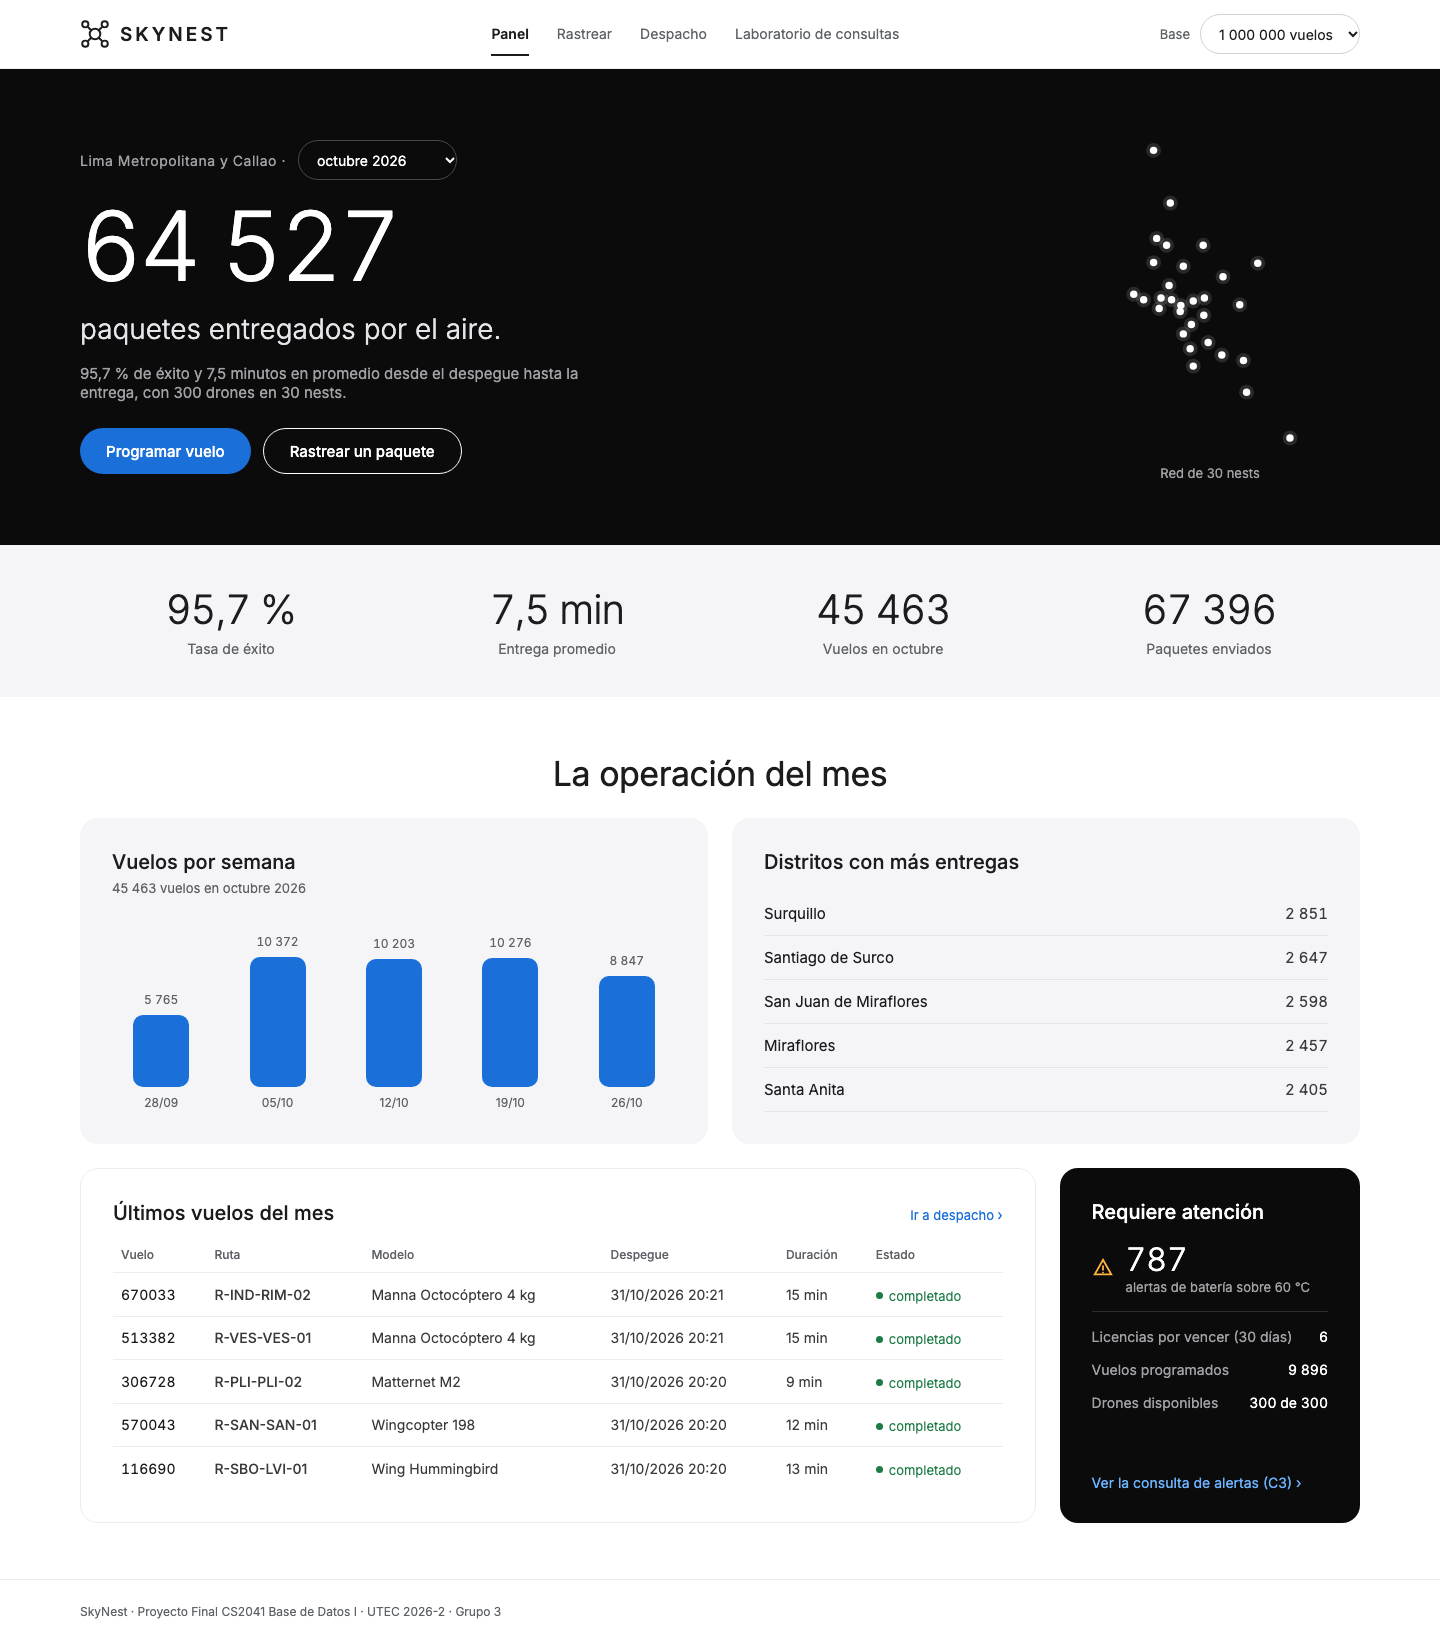
\includegraphics[width=0.85\linewidth,height=0.8\textheight,keepaspectratio]{capturas/01_panel.png}
\caption{Panel con la base de 1\,000\,000 de vuelos (octubre de 2026)}
\end{figure}

\begin{figure}[H]\centering
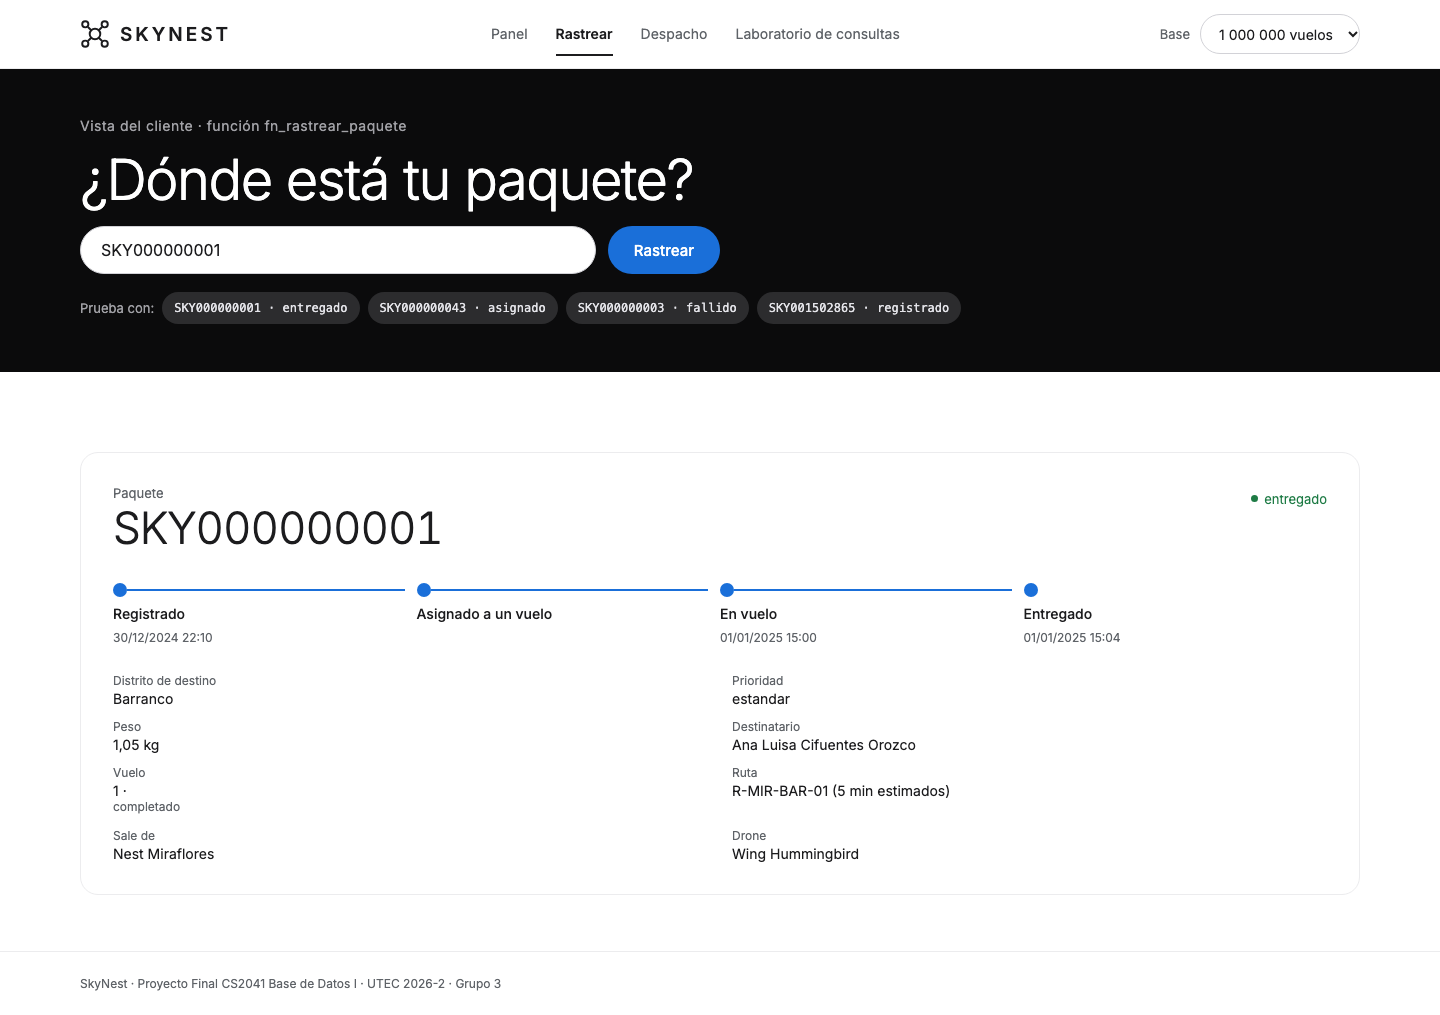
\includegraphics[width=0.85\linewidth,height=0.8\textheight,keepaspectratio]{capturas/02_rastrear.png}
\caption{Rastreo de un paquete con \at{fn\_rastrear\_paquete}}
\end{figure}

\begin{figure}[H]\centering
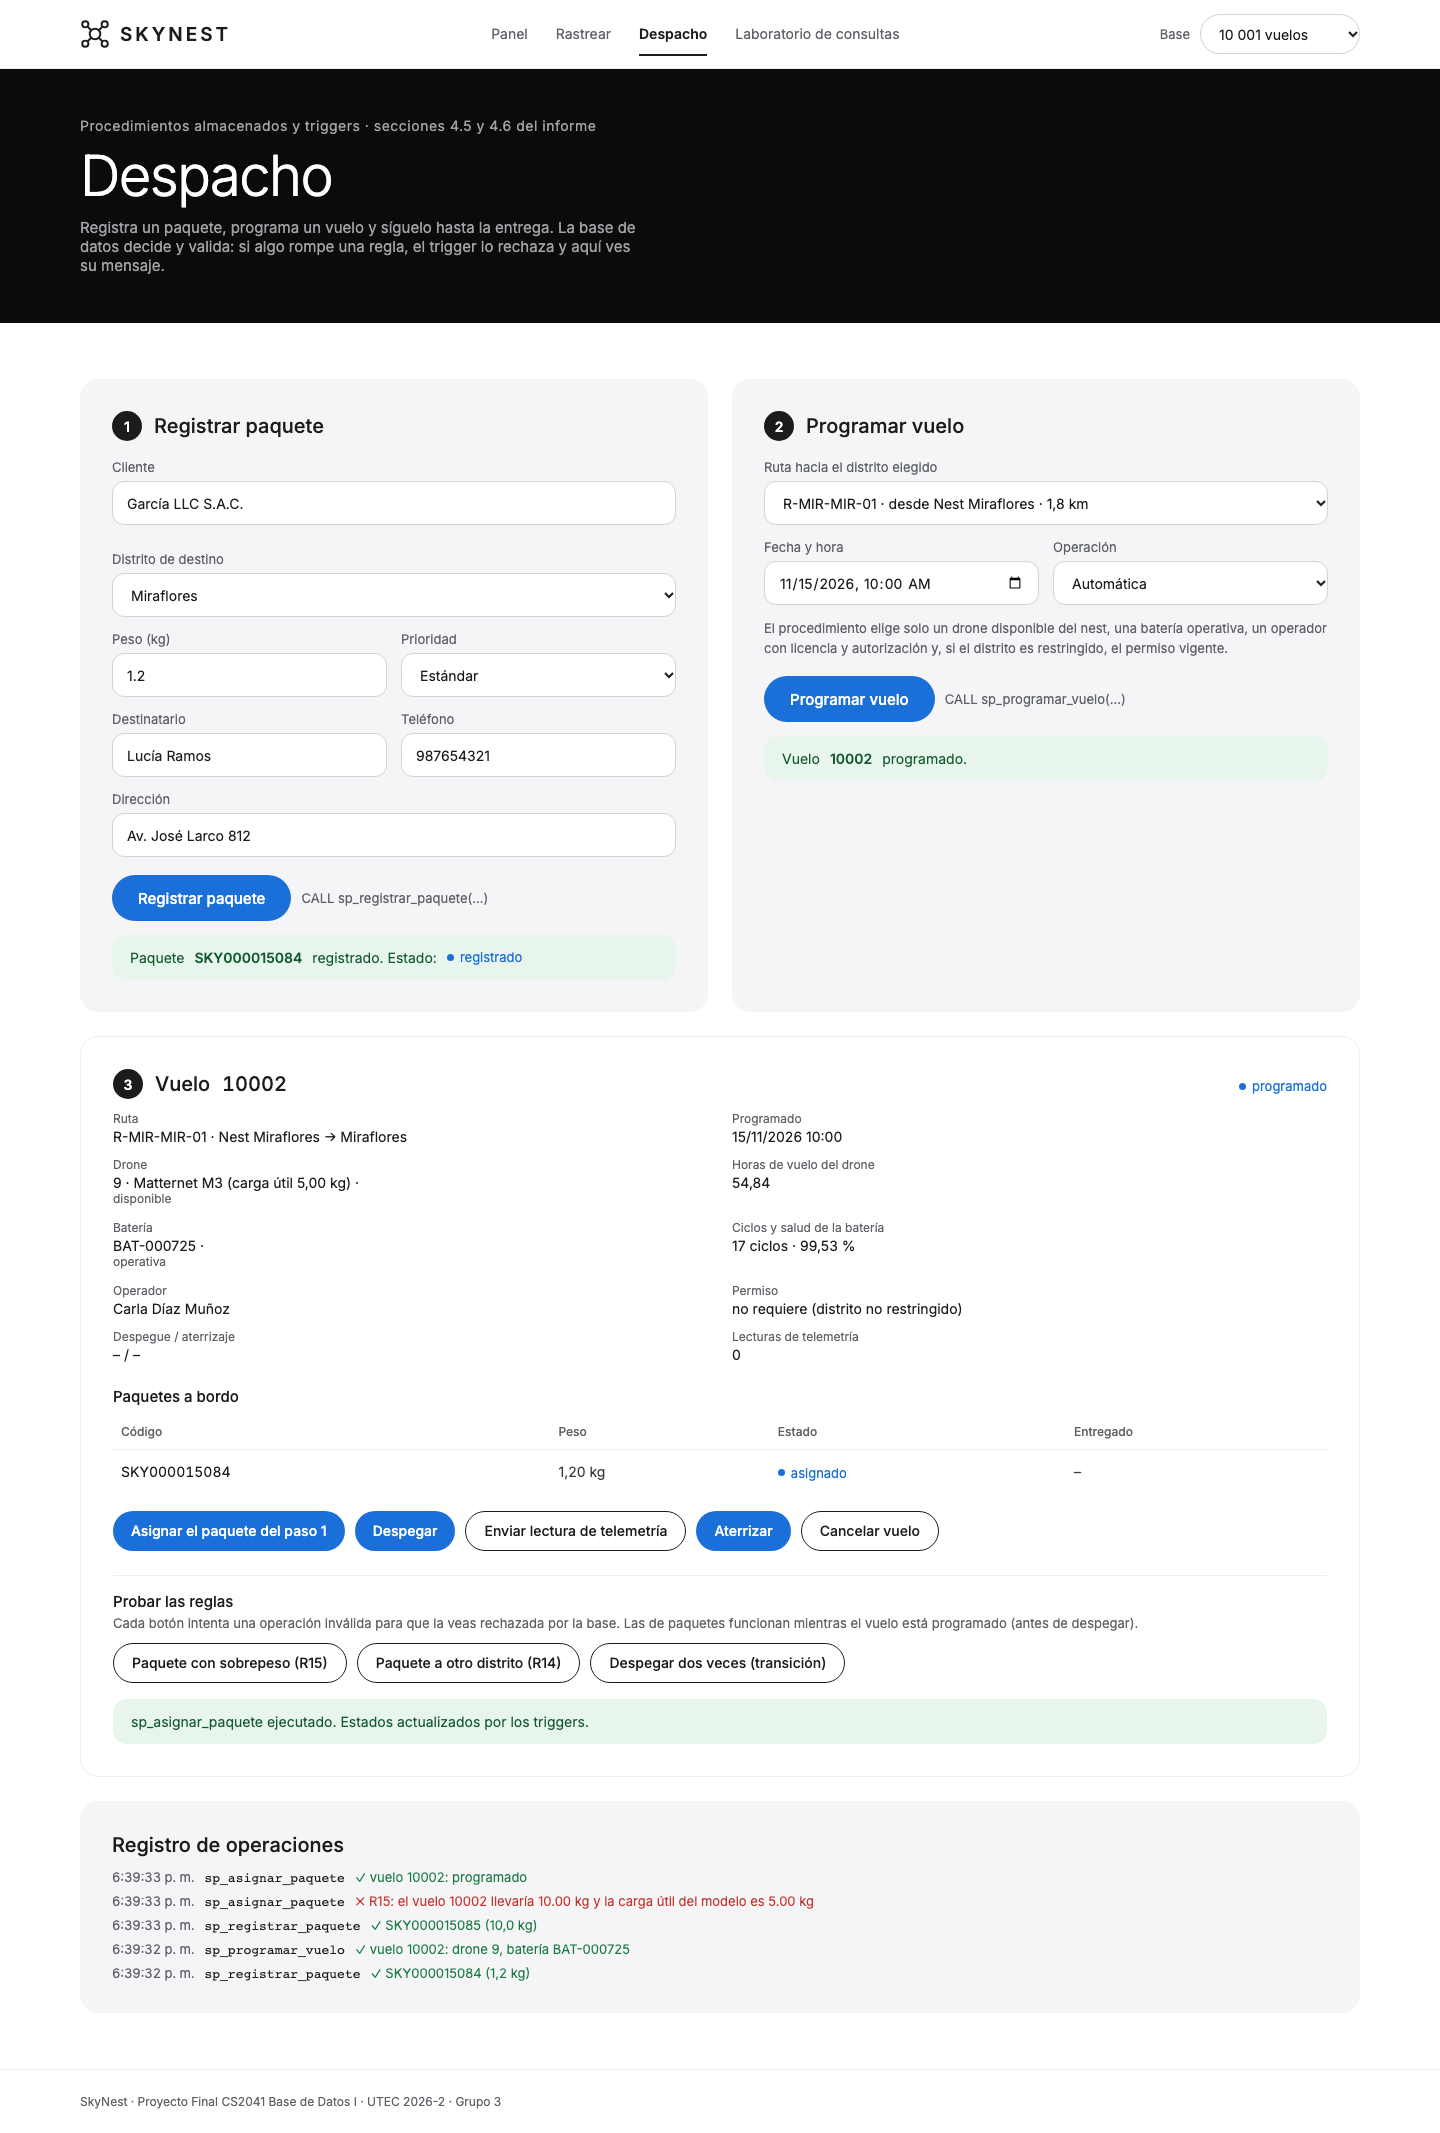
\includegraphics[width=0.85\linewidth,height=0.8\textheight,keepaspectratio]{capturas/03_despacho.png}
\caption{Despacho: paquete registrado, vuelo programado y asignación. En el registro de operaciones se ve el rechazo del trigger de R15 (paquete con sobrepeso).}
\end{figure}

\begin{figure}[H]\centering
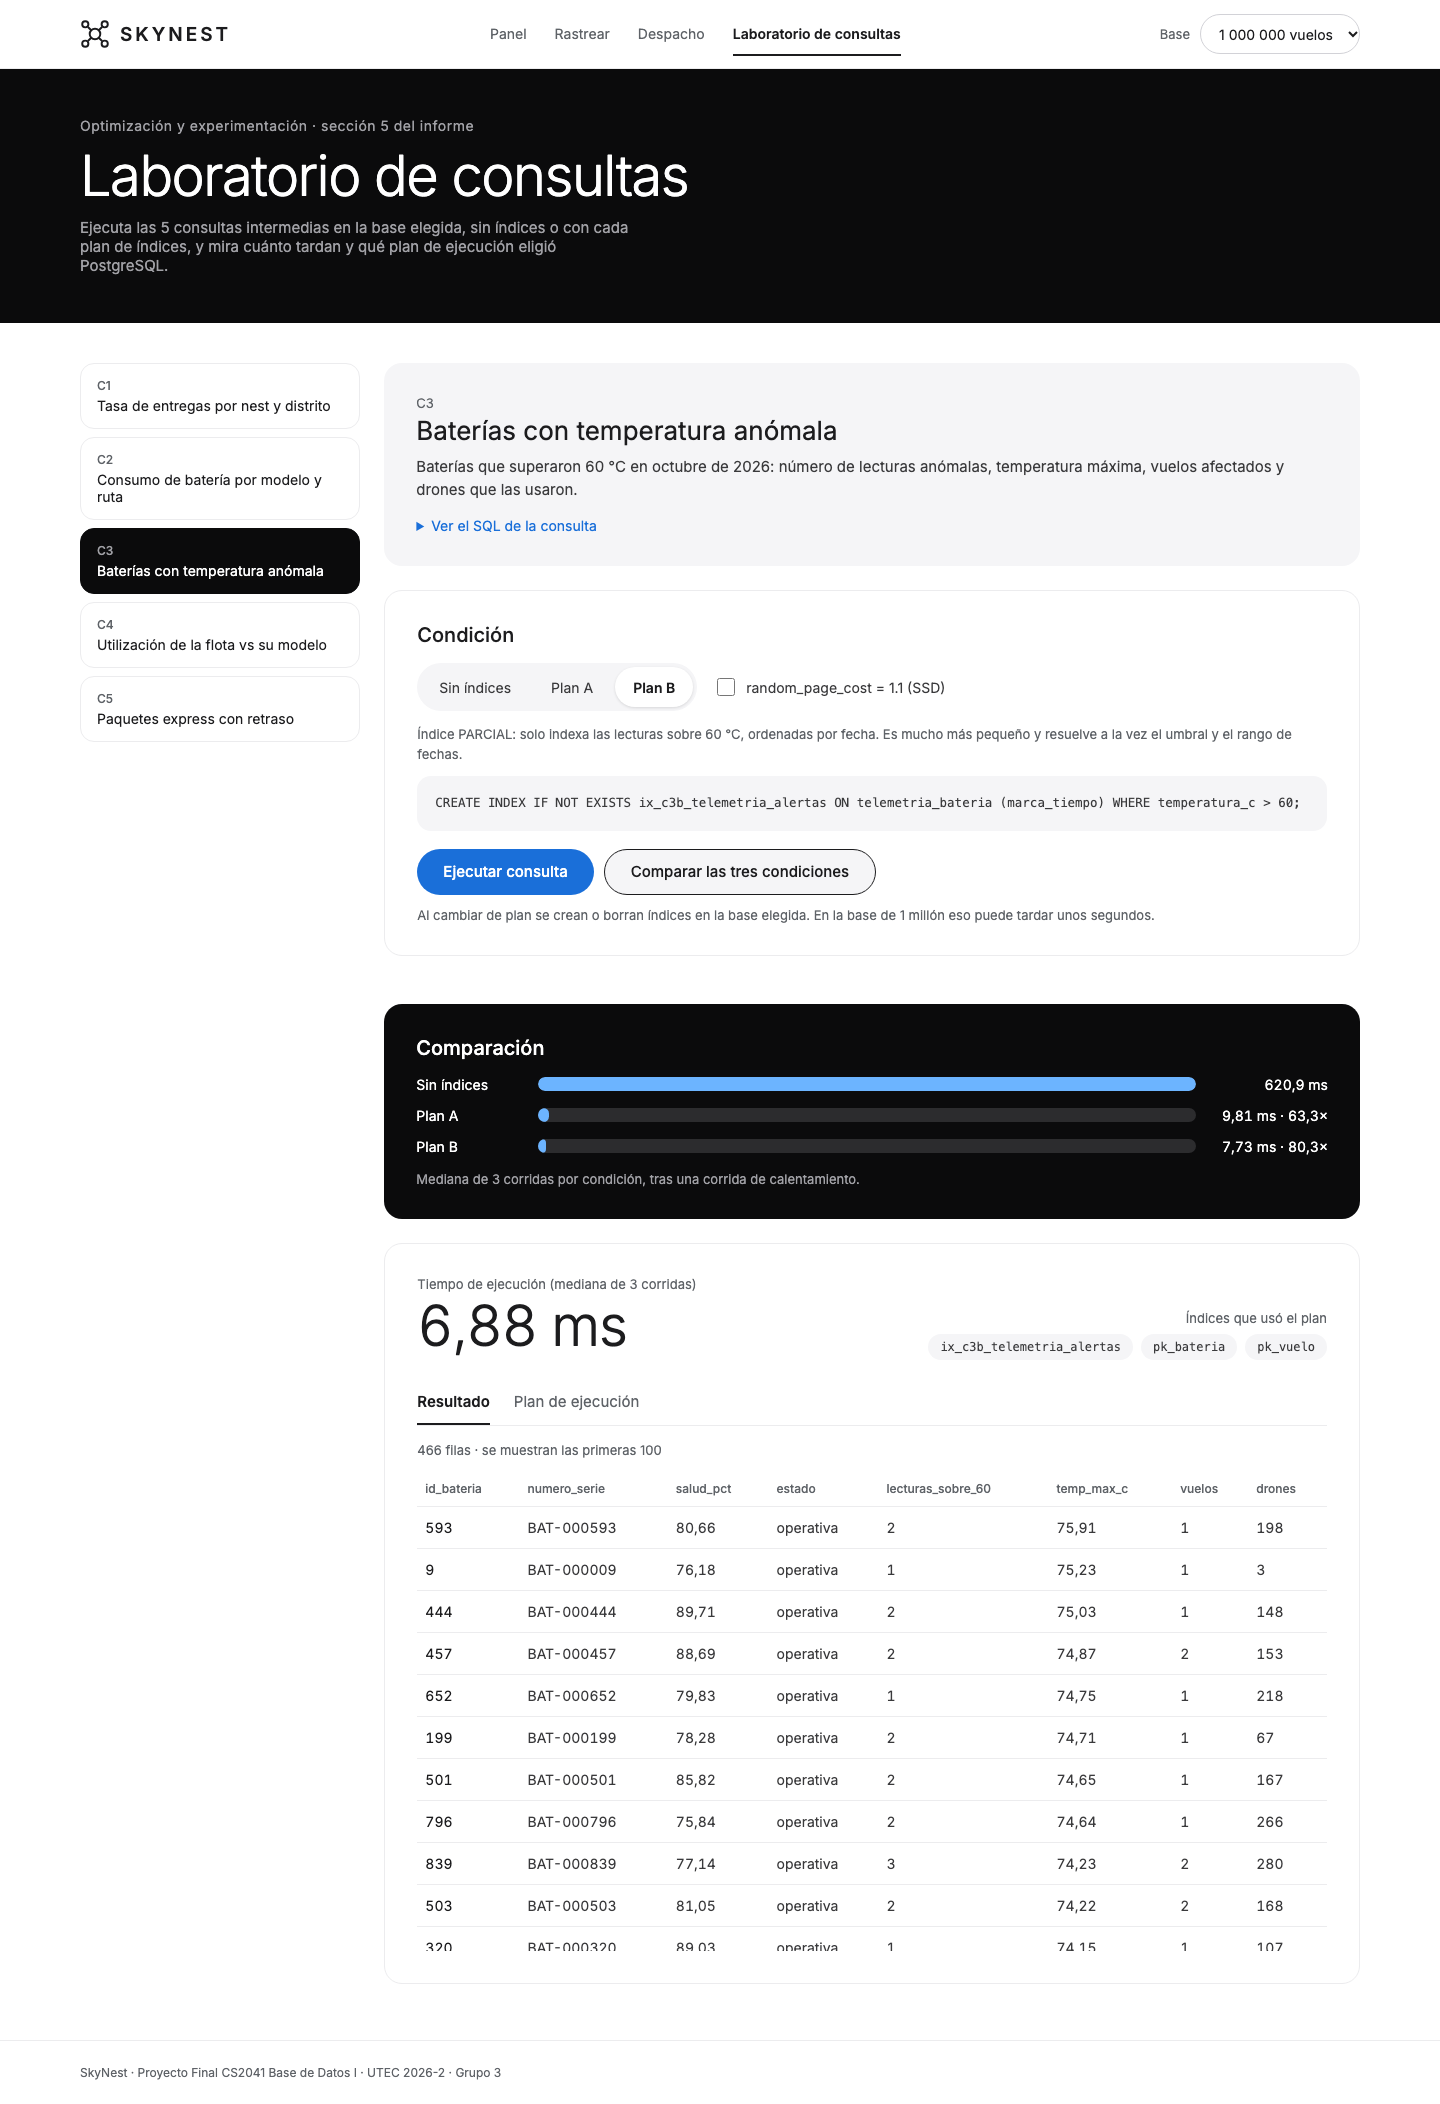
\includegraphics[width=0.85\linewidth,height=0.8\textheight,keepaspectratio]{capturas/04_laboratorio.png}
\caption{Laboratorio: C3 con el plan B y la comparación de las tres condiciones en la base de 1\,000\,000 de vuelos}
\end{figure}

\begin{figure}[H]\centering
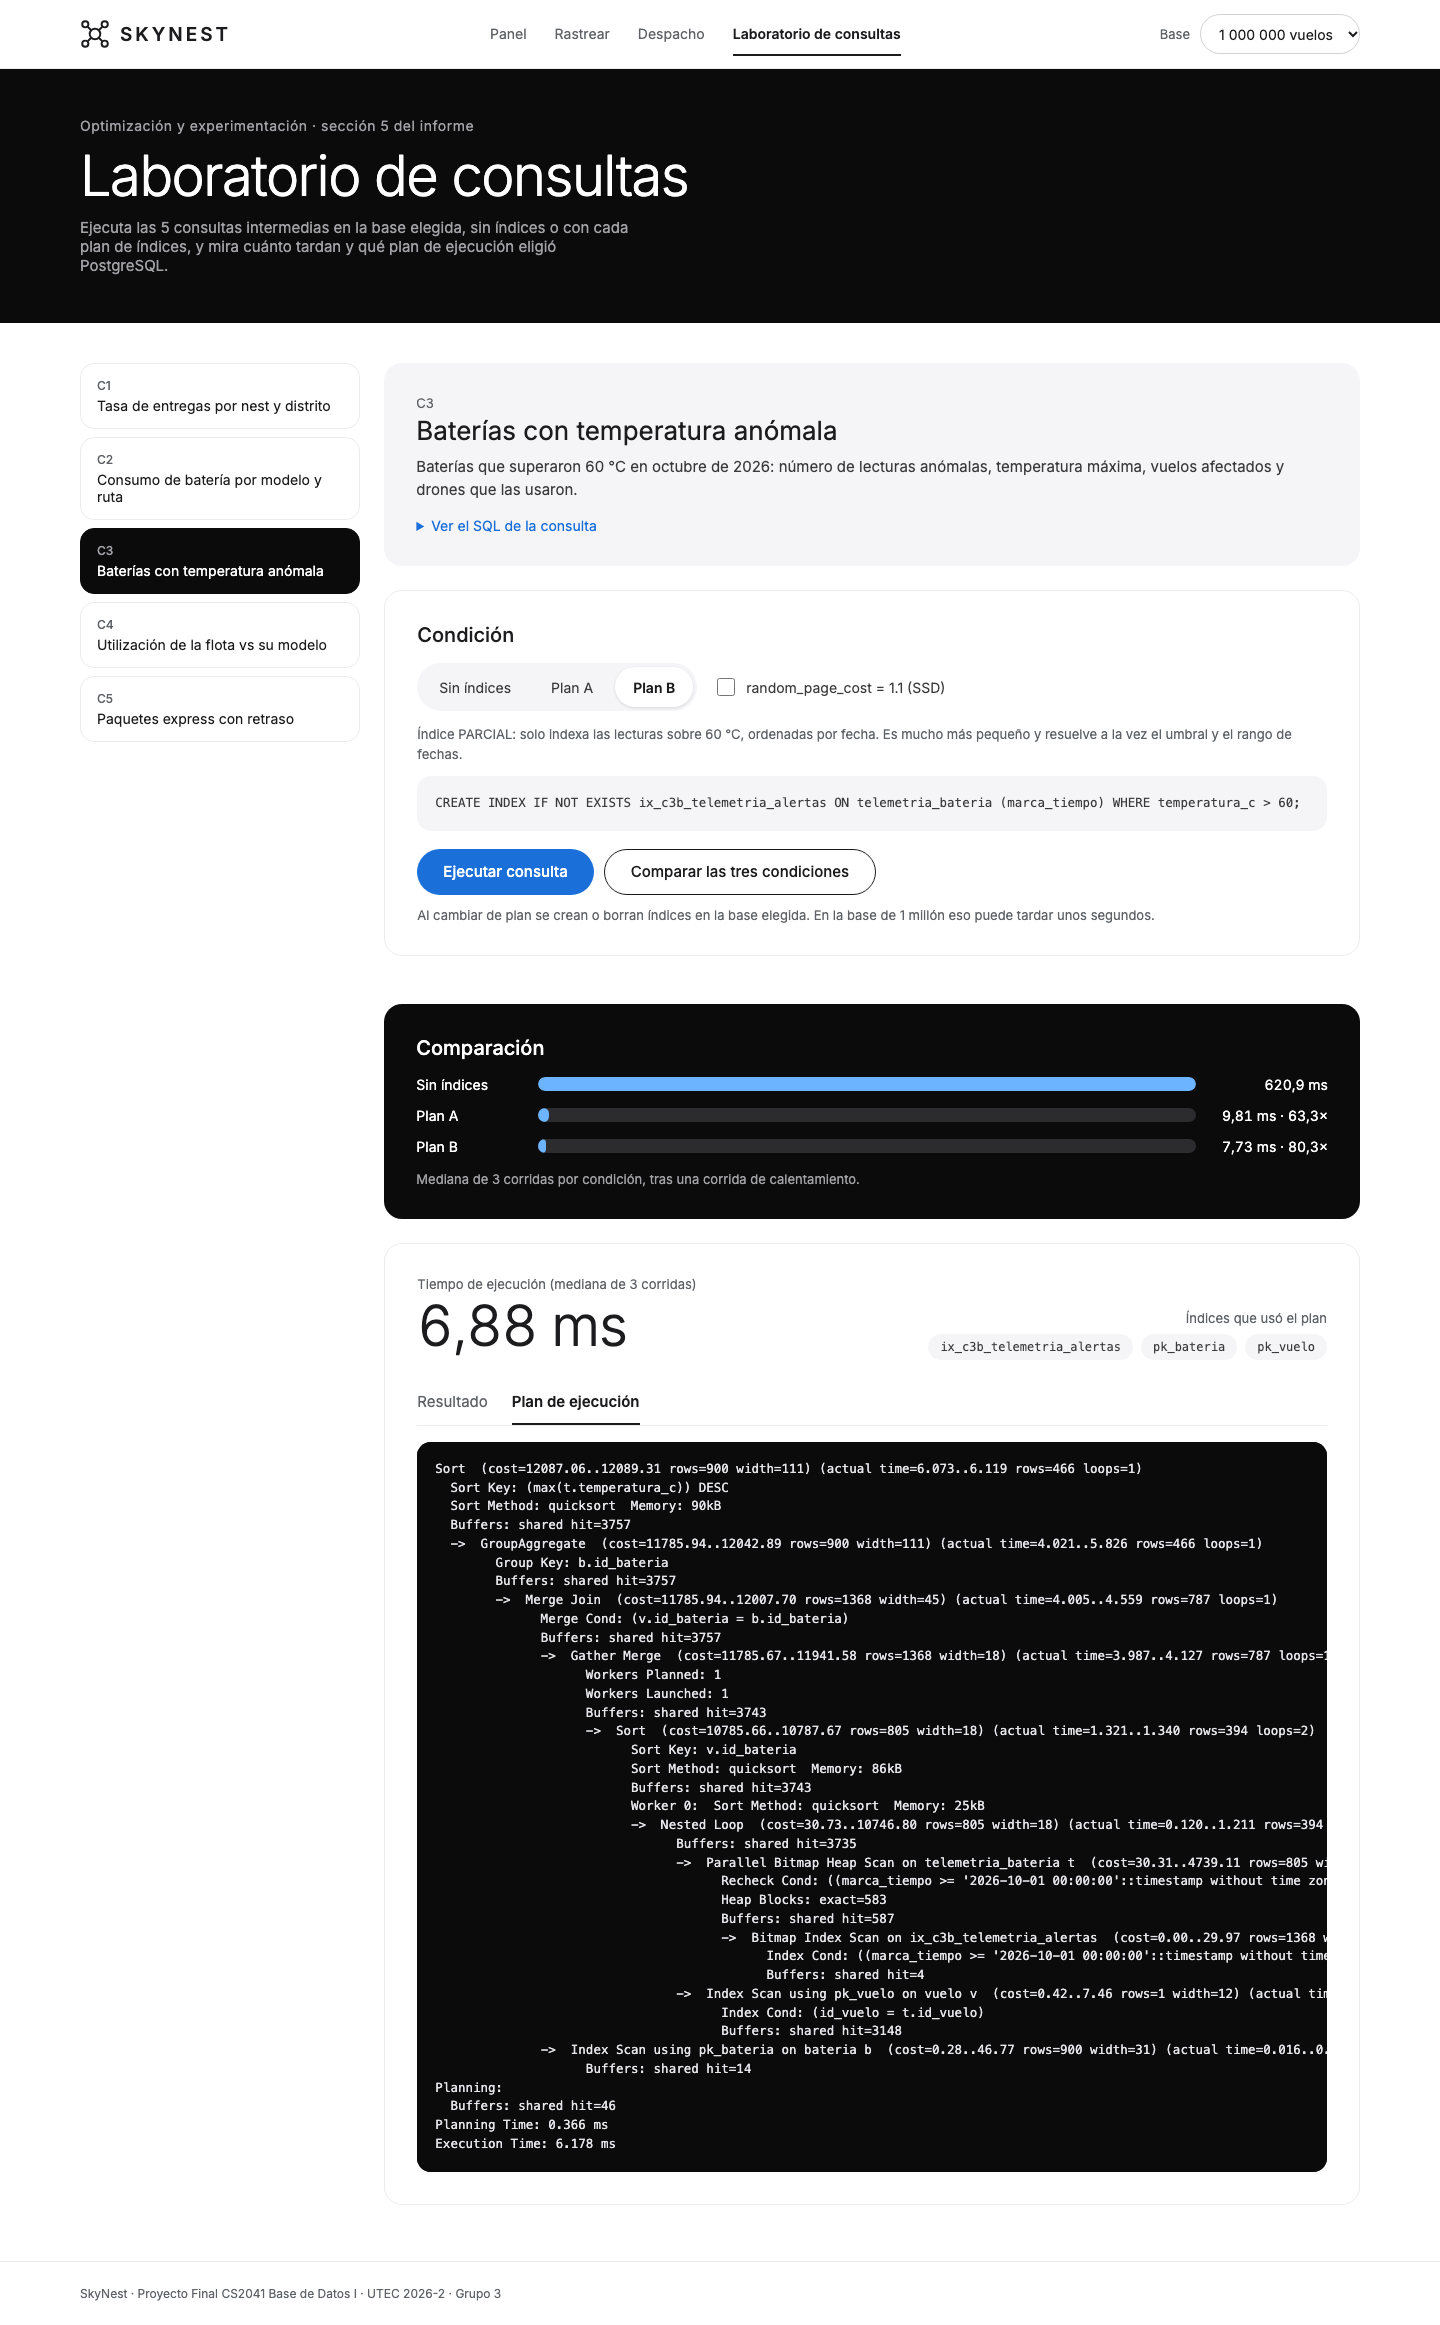
\includegraphics[width=0.85\linewidth,height=0.8\textheight,keepaspectratio]{capturas/05_laboratorio_plan.png}
\caption{Laboratorio: plan de ejecución de C3 con el índice parcial}
\end{figure}

\subsection{Video de la experimentación}
Cinco videos, uno por consulta, ejecutados en pgAdmin sobre la base de 1\,000\,000 de vuelos. Cada uno muestra el plan de ejecución y el tiempo de la consulta sin índices y con el índice que más la mejoró, y al final borra el índice. Los scripts están en \archivo{video_ejemplo/demo_c1.sql} a \archivo{video_ejemplo/demo_c5.sql}.
\begin{itemize}
\item Consulta 1 (índices cubrientes): \url{https://drive.google.com/file/d/1DEceSLNMxklyqunQvqVqOuqCeRu2gj0q/view?usp=sharing}
\item Consulta 2 (índice compuesto): \url{https://drive.google.com/file/d/1Z0WbNbNy_PGJT4Hyp_flKM138V4MB763/view?usp=sharing}
\item Consulta 3 (índice parcial): \url{https://drive.google.com/file/d/1_n6P6XFe2Ad9zzlDHDcNQMmzZyukfyrT/view?usp=sharing}
\item Consulta 4 (B+ en la fecha): \url{https://drive.google.com/file/d/1BN2_Bi6wa98XnyDzW_MDW-j1pnpCZ0Bc/view?usp=sharing}
\item Consulta 5 (compuesto y cubriente, y \texttt{random\_page\_cost = 1.1}): \url{https://drive.google.com/file/d/13Pmu5ubarhSRa7YgPcjhtEzehZe1QTMF/view?usp=sharing}
\end{itemize}

% ---------------------------------------------------------------------
\subsection{Repositorio del proyecto}
\label{sec:repositorio}
Todos los archivos del proyecto están en el repositorio público \url{https://github.com/gdny0208/Proyecto-Final-Skynest}, incluidos los cuatro dumps del experimento (con Git LFS, porque el de 1M supera el límite de 100\,MB por archivo de GitHub). El archivo \archivo{README.md} explica cómo instalarlo, restaurar las bases y repetir el experimento.

\begin{table}[H]
\centering\small
\caption{Contenido del repositorio}
\label{tab:repo}
\begin{tabularx}{\linewidth}{@{}>{\raggedright\arraybackslash}p{4.4cm}>{\raggedright\arraybackslash}X@{}}
\toprule
Carpeta & Contenido \\
\midrule
\archivo{sql/} & scripts 01 a 08 (esquemas y tablas, datos reales, triggers, procedimientos, vistas, roles, consultas e índices) y sus pruebas \\
\archivo{gen/} & generador de datos sintéticos, verificación de las 18 reglas y construcción de las 4 bases \\
\archivo{bench/} & programa del experimento (sección~\ref{sec:metodologia}) \\
\archivo{dumps/} & los 4 dumps: \archivo{skynest_1k.dump} a \archivo{skynest_1m.dump} (Git LFS) \\
\archivo{informe/resultados/} & tiempos de todas las corridas (CSV), los 80 planes de ejecución, gráficos y tablas \\
\archivo{informe/evidencias/} & salidas de la construcción de las bases, las pruebas y el experimento \\
\archivo{video_ejemplo/} & scripts que se ejecutan en los 5 videos (\archivo{demo_c1.sql} a \archivo{demo_c5.sql}) \\
\archivo{web/} & MVP web (FastAPI y PostgreSQL), sección~\ref{sec:mvp} \\
\archivo{docs/} & informe y modelo E/R del Hito 1 \\
\bottomrule
\end{tabularx}
\end{table}

% ---------------------------------------------------------------------
\subsection{Planes de ejecución completos (escala 1M)}
\label{sec:planes_completos}
Salida completa de \texttt{EXPLAIN (ANALYZE, BUFFERS)} de los planes resumidos en la sección~\ref{sec:planes}. Los 80 planes (4 escalas, 5 consultas y 4 condiciones) están en \archivo{informe/resultados/planes/}.

\subsubsection*{Consulta 1}
\textbf{Sin índices:}\plan{1m_C1_sin.txt}
\textbf{Plan B:}\plan{1m_C1_B.txt}
\subsubsection*{Consulta 2}
\textbf{Sin índices:}\plan{1m_C2_sin.txt}
\textbf{Plan A:}\plan{1m_C2_A.txt}
\subsubsection*{Consulta 3}
\textbf{Sin índices:}\plan{1m_C3_sin.txt}
\textbf{Plan B:}\plan{1m_C3_B.txt}
\subsubsection*{Consulta 4}
\textbf{Sin índices:}\plan{1m_C4_sin.txt}
\textbf{Plan A:}\plan{1m_C4_A.txt}
\subsubsection*{Consulta 5}
\textbf{Plan B:}\plan{1m_C5_B.txt}
\textbf{Plan B con \texttt{random\_page\_cost = 1.1}:}\plan{1m_C5_B_rpc.txt}

\subsection{Dumps y scripts}
Los cuatro dumps (\archivo{skynest_1k.dump}, \archivo{skynest_10k.dump}, \archivo{skynest_100k.dump} y \archivo{skynest_1m.dump}) están en la carpeta \archivo{dumps/} del repositorio (sección~\ref{sec:repositorio}). Se descargan desde la web de GitHub (botón \emph{Download} de cada archivo, \url{https://github.com/gdny0208/Proyecto-Final-Skynest/tree/main/dumps}) o, después de clonar el repositorio, con \texttt{git lfs pull}. Se restauran con:
\begin{lstlisting}[style=salida]
createdb skynest_1m && pg_restore -d skynest_1m dumps/skynest_1m.dump
psql -d skynest_1m -c "ALTER DATABASE skynest_1m SET search_path = skynest, reportes, public"
\end{lstlisting}
La segunda línea se necesita porque \texttt{pg\_dump} guarda los esquemas y su contenido, pero no la ruta de búsqueda por defecto de la base.
Para reconstruir todo desde cero (bases, verificación, dumps) y repetir el experimento:
\begin{lstlisting}[style=salida]
bash gen/construir_bases.sh                  # 4 bases + 4 dumps
.venv/bin/python bench/experimento.py        # tablas, gráficos y planes en informe/resultados/
\end{lstlisting}


\end{document}
